\documentclass[twoside]{book}

% Packages required by doxygen
\usepackage{fixltx2e}
\usepackage{calc}
\usepackage{doxygen}
\usepackage[export]{adjustbox} % also loads graphicx
\usepackage{graphicx}
\usepackage[utf8]{inputenc}
\usepackage{makeidx}
\usepackage{multicol}
\usepackage{multirow}
\PassOptionsToPackage{warn}{textcomp}
\usepackage{textcomp}
\usepackage[nointegrals]{wasysym}
\usepackage[table]{xcolor}

% Font selection
\usepackage[T1]{fontenc}
\usepackage[scaled=.90]{helvet}
\usepackage{courier}
\usepackage{amssymb}
\usepackage{sectsty}
\renewcommand{\familydefault}{\sfdefault}
\allsectionsfont{%
  \fontseries{bc}\selectfont%
  \color{darkgray}%
}
\renewcommand{\DoxyLabelFont}{%
  \fontseries{bc}\selectfont%
  \color{darkgray}%
}
\newcommand{\+}{\discretionary{\mbox{\scriptsize$\hookleftarrow$}}{}{}}

% Page & text layout
\usepackage{geometry}
\geometry{%
  a4paper,%
  top=2.5cm,%
  bottom=2.5cm,%
  left=2.5cm,%
  right=2.5cm%
}
\tolerance=750
\hfuzz=15pt
\hbadness=750
\setlength{\emergencystretch}{15pt}
\setlength{\parindent}{0cm}
\setlength{\parskip}{3ex plus 2ex minus 2ex}
\makeatletter
\renewcommand{\paragraph}{%
  \@startsection{paragraph}{4}{0ex}{-1.0ex}{1.0ex}{%
    \normalfont\normalsize\bfseries\SS@parafont%
  }%
}
\renewcommand{\subparagraph}{%
  \@startsection{subparagraph}{5}{0ex}{-1.0ex}{1.0ex}{%
    \normalfont\normalsize\bfseries\SS@subparafont%
  }%
}
\makeatother

% Headers & footers
\usepackage{fancyhdr}
\pagestyle{fancyplain}
\fancyhead[LE]{\fancyplain{}{\bfseries\thepage}}
\fancyhead[CE]{\fancyplain{}{}}
\fancyhead[RE]{\fancyplain{}{\bfseries\leftmark}}
\fancyhead[LO]{\fancyplain{}{\bfseries\rightmark}}
\fancyhead[CO]{\fancyplain{}{}}
\fancyhead[RO]{\fancyplain{}{\bfseries\thepage}}
\fancyfoot[LE]{\fancyplain{}{}}
\fancyfoot[CE]{\fancyplain{}{}}
\fancyfoot[RE]{\fancyplain{}{\bfseries\scriptsize Generated by Doxygen }}
\fancyfoot[LO]{\fancyplain{}{\bfseries\scriptsize Generated by Doxygen }}
\fancyfoot[CO]{\fancyplain{}{}}
\fancyfoot[RO]{\fancyplain{}{}}
\renewcommand{\footrulewidth}{0.4pt}
\renewcommand{\chaptermark}[1]{%
  \markboth{#1}{}%
}
\renewcommand{\sectionmark}[1]{%
  \markright{\thesection\ #1}%
}

% Indices & bibliography
\usepackage{natbib}
\usepackage[titles]{tocloft}
\setcounter{tocdepth}{3}
\setcounter{secnumdepth}{5}
\makeindex

% Hyperlinks (required, but should be loaded last)
\usepackage{ifpdf}
\ifpdf
  \usepackage[pdftex,pagebackref=true]{hyperref}
\else
  \usepackage[ps2pdf,pagebackref=true]{hyperref}
\fi
\hypersetup{%
  colorlinks=true,%
  linkcolor=blue,%
  citecolor=blue,%
  unicode%
}

% Custom commands
\newcommand{\clearemptydoublepage}{%
  \newpage{\pagestyle{empty}\cleardoublepage}%
}

\usepackage{caption}
\captionsetup{labelsep=space,justification=centering,font={bf},singlelinecheck=off,skip=4pt,position=top}

%===== C O N T E N T S =====

\begin{document}

% Titlepage & ToC
\hypersetup{pageanchor=false,
             bookmarksnumbered=true,
             pdfencoding=unicode
            }
\pagenumbering{alph}
\begin{titlepage}
\vspace*{7cm}
\begin{center}%
{\Large employee\+Directory }\\
\vspace*{1cm}
{\large Generated by Doxygen 1.8.14}\\
\end{center}
\end{titlepage}
\clearemptydoublepage
\pagenumbering{roman}
\tableofcontents
\clearemptydoublepage
\pagenumbering{arabic}
\hypersetup{pageanchor=true}

%--- Begin generated contents ---
\chapter{Hierarchical Index}
\section{Class Hierarchy}
This inheritance list is sorted roughly, but not completely, alphabetically\+:\begin{DoxyCompactList}
\item Base\+User\begin{DoxyCompactList}
\item \contentsline{section}{App\+Bundle\textbackslash{}Entity\textbackslash{}User}{\pageref{class_app_bundle_1_1_entity_1_1_user}}{}
\end{DoxyCompactList}
\item \contentsline{section}{App\+Bundle\textbackslash{}Entity\textbackslash{}Employee}{\pageref{class_app_bundle_1_1_entity_1_1_employee}}{}
\item Entity\+Repository\begin{DoxyCompactList}
\item \contentsline{section}{App\+Bundle\textbackslash{}Repository\textbackslash{}Employee\+Repository}{\pageref{class_app_bundle_1_1_repository_1_1_employee_repository}}{}
\item \contentsline{section}{App\+Bundle\textbackslash{}Repository\textbackslash{}Environment\+Repository}{\pageref{class_app_bundle_1_1_repository_1_1_environment_repository}}{}
\item \contentsline{section}{App\+Bundle\textbackslash{}Repository\textbackslash{}Skills\+Repository}{\pageref{class_app_bundle_1_1_repository_1_1_skills_repository}}{}
\end{DoxyCompactList}
\item \contentsline{section}{App\+Bundle\textbackslash{}Entity\textbackslash{}Environment}{\pageref{class_app_bundle_1_1_entity_1_1_environment}}{}
\item \contentsline{section}{App\+Bundle\textbackslash{}Entity\textbackslash{}Skill}{\pageref{class_app_bundle_1_1_entity_1_1_skill}}{}
\item Abstract\+Type\begin{DoxyCompactList}
\item \contentsline{section}{App\+Bundle\textbackslash{}Form\textbackslash{}Employee\+Type}{\pageref{class_app_bundle_1_1_form_1_1_employee_type}}{}
\item \contentsline{section}{App\+Bundle\textbackslash{}Form\textbackslash{}Environment\+Type}{\pageref{class_app_bundle_1_1_form_1_1_environment_type}}{}
\item \contentsline{section}{App\+Bundle\textbackslash{}Form\textbackslash{}Skill\+Type}{\pageref{class_app_bundle_1_1_form_1_1_skill_type}}{}
\end{DoxyCompactList}
\item Bundle\begin{DoxyCompactList}
\item \contentsline{section}{App\+Bundle\textbackslash{}App\+Bundle}{\pageref{class_app_bundle_1_1_app_bundle}}{}
\end{DoxyCompactList}
\item Controller\begin{DoxyCompactList}
\item \contentsline{section}{App\+Bundle\textbackslash{}Controller\textbackslash{}Add\+Controller}{\pageref{class_app_bundle_1_1_controller_1_1_add_controller}}{}
\item \contentsline{section}{App\+Bundle\textbackslash{}Controller\textbackslash{}A\+P\+I\+Controller}{\pageref{class_app_bundle_1_1_controller_1_1_a_p_i_controller}}{}
\item \contentsline{section}{App\+Bundle\textbackslash{}Controller\textbackslash{}Delete\+Controller}{\pageref{class_app_bundle_1_1_controller_1_1_delete_controller}}{}
\item \contentsline{section}{App\+Bundle\textbackslash{}Controller\textbackslash{}Details\+Controller}{\pageref{class_app_bundle_1_1_controller_1_1_details_controller}}{}
\item \contentsline{section}{App\+Bundle\textbackslash{}Controller\textbackslash{}Edit\+Controller}{\pageref{class_app_bundle_1_1_controller_1_1_edit_controller}}{}
\item \contentsline{section}{App\+Bundle\textbackslash{}Controller\textbackslash{}Employee\+Controller}{\pageref{class_app_bundle_1_1_controller_1_1_employee_controller}}{}
\item \contentsline{section}{App\+Bundle\textbackslash{}Controller\textbackslash{}List\+Controller}{\pageref{class_app_bundle_1_1_controller_1_1_list_controller}}{}
\item \contentsline{section}{App\+Bundle\textbackslash{}Controller\textbackslash{}Login\+Controller}{\pageref{class_app_bundle_1_1_controller_1_1_login_controller}}{}
\item \contentsline{section}{App\+Bundle\textbackslash{}Controller\textbackslash{}Logout\+Controller}{\pageref{class_app_bundle_1_1_controller_1_1_logout_controller}}{}
\end{DoxyCompactList}
\item Web\+Test\+Case\begin{DoxyCompactList}
\item \contentsline{section}{App\+Bundle\textbackslash{}Tests\textbackslash{}Controller\textbackslash{}A\+P\+I\+Controller\+Test}{\pageref{class_app_bundle_1_1_tests_1_1_controller_1_1_a_p_i_controller_test}}{}
\item \contentsline{section}{App\+Bundle\textbackslash{}Tests\textbackslash{}Controller\textbackslash{}Delete\+Controller\+Controller\+Test}{\pageref{class_app_bundle_1_1_tests_1_1_controller_1_1_delete_controller_controller_test}}{}
\item \contentsline{section}{App\+Bundle\textbackslash{}Tests\textbackslash{}Controller\textbackslash{}Details\+Controller\+Controller\+Test}{\pageref{class_app_bundle_1_1_tests_1_1_controller_1_1_details_controller_controller_test}}{}
\item \contentsline{section}{App\+Bundle\textbackslash{}Tests\textbackslash{}Controller\textbackslash{}Edit\+Controller\+Controller\+Test}{\pageref{class_app_bundle_1_1_tests_1_1_controller_1_1_edit_controller_controller_test}}{}
\item \contentsline{section}{App\+Bundle\textbackslash{}Tests\textbackslash{}Controller\textbackslash{}Employee\+Controller\+Test}{\pageref{class_app_bundle_1_1_tests_1_1_controller_1_1_employee_controller_test}}{}
\item \contentsline{section}{App\+Bundle\textbackslash{}Tests\textbackslash{}Controller\textbackslash{}Login\+Controller\+Test}{\pageref{class_app_bundle_1_1_tests_1_1_controller_1_1_login_controller_test}}{}
\item \contentsline{section}{App\+Bundle\textbackslash{}Tests\textbackslash{}Controller\textbackslash{}Logout\+Controller\+Test}{\pageref{class_app_bundle_1_1_tests_1_1_controller_1_1_logout_controller_test}}{}
\end{DoxyCompactList}
\end{DoxyCompactList}

\chapter{Class Index}
\section{Class List}
Here are the classes, structs, unions and interfaces with brief descriptions\+:\begin{DoxyCompactList}
\item\contentsline{section}{\mbox{\hyperlink{class_app_bundle_1_1_controller_1_1_add_controller}{App\+Bundle\textbackslash{}\+Controller\textbackslash{}\+Add\+Controller}} }{\pageref{class_app_bundle_1_1_controller_1_1_add_controller}}{}
\item\contentsline{section}{\mbox{\hyperlink{class_app_bundle_1_1_controller_1_1_a_p_i_controller}{App\+Bundle\textbackslash{}\+Controller\textbackslash{}\+A\+P\+I\+Controller}} }{\pageref{class_app_bundle_1_1_controller_1_1_a_p_i_controller}}{}
\item\contentsline{section}{\mbox{\hyperlink{class_app_bundle_1_1_tests_1_1_controller_1_1_a_p_i_controller_test}{App\+Bundle\textbackslash{}\+Tests\textbackslash{}\+Controller\textbackslash{}\+A\+P\+I\+Controller\+Test}} }{\pageref{class_app_bundle_1_1_tests_1_1_controller_1_1_a_p_i_controller_test}}{}
\item\contentsline{section}{\mbox{\hyperlink{class_app_bundle_1_1_app_bundle}{App\+Bundle\textbackslash{}\+App\+Bundle}} }{\pageref{class_app_bundle_1_1_app_bundle}}{}
\item\contentsline{section}{\mbox{\hyperlink{class_app_bundle_1_1_controller_1_1_delete_controller}{App\+Bundle\textbackslash{}\+Controller\textbackslash{}\+Delete\+Controller}} }{\pageref{class_app_bundle_1_1_controller_1_1_delete_controller}}{}
\item\contentsline{section}{\mbox{\hyperlink{class_app_bundle_1_1_tests_1_1_controller_1_1_delete_controller_controller_test}{App\+Bundle\textbackslash{}\+Tests\textbackslash{}\+Controller\textbackslash{}\+Delete\+Controller\+Controller\+Test}} }{\pageref{class_app_bundle_1_1_tests_1_1_controller_1_1_delete_controller_controller_test}}{}
\item\contentsline{section}{\mbox{\hyperlink{class_app_bundle_1_1_controller_1_1_details_controller}{App\+Bundle\textbackslash{}\+Controller\textbackslash{}\+Details\+Controller}} }{\pageref{class_app_bundle_1_1_controller_1_1_details_controller}}{}
\item\contentsline{section}{\mbox{\hyperlink{class_app_bundle_1_1_tests_1_1_controller_1_1_details_controller_controller_test}{App\+Bundle\textbackslash{}\+Tests\textbackslash{}\+Controller\textbackslash{}\+Details\+Controller\+Controller\+Test}} }{\pageref{class_app_bundle_1_1_tests_1_1_controller_1_1_details_controller_controller_test}}{}
\item\contentsline{section}{\mbox{\hyperlink{class_app_bundle_1_1_controller_1_1_edit_controller}{App\+Bundle\textbackslash{}\+Controller\textbackslash{}\+Edit\+Controller}} }{\pageref{class_app_bundle_1_1_controller_1_1_edit_controller}}{}
\item\contentsline{section}{\mbox{\hyperlink{class_app_bundle_1_1_tests_1_1_controller_1_1_edit_controller_controller_test}{App\+Bundle\textbackslash{}\+Tests\textbackslash{}\+Controller\textbackslash{}\+Edit\+Controller\+Controller\+Test}} }{\pageref{class_app_bundle_1_1_tests_1_1_controller_1_1_edit_controller_controller_test}}{}
\item\contentsline{section}{\mbox{\hyperlink{class_app_bundle_1_1_entity_1_1_employee}{App\+Bundle\textbackslash{}\+Entity\textbackslash{}\+Employee}} }{\pageref{class_app_bundle_1_1_entity_1_1_employee}}{}
\item\contentsline{section}{\mbox{\hyperlink{class_app_bundle_1_1_controller_1_1_employee_controller}{App\+Bundle\textbackslash{}\+Controller\textbackslash{}\+Employee\+Controller}} }{\pageref{class_app_bundle_1_1_controller_1_1_employee_controller}}{}
\item\contentsline{section}{\mbox{\hyperlink{class_app_bundle_1_1_tests_1_1_controller_1_1_employee_controller_test}{App\+Bundle\textbackslash{}\+Tests\textbackslash{}\+Controller\textbackslash{}\+Employee\+Controller\+Test}} }{\pageref{class_app_bundle_1_1_tests_1_1_controller_1_1_employee_controller_test}}{}
\item\contentsline{section}{\mbox{\hyperlink{class_app_bundle_1_1_repository_1_1_employee_repository}{App\+Bundle\textbackslash{}\+Repository\textbackslash{}\+Employee\+Repository}} }{\pageref{class_app_bundle_1_1_repository_1_1_employee_repository}}{}
\item\contentsline{section}{\mbox{\hyperlink{class_app_bundle_1_1_form_1_1_employee_type}{App\+Bundle\textbackslash{}\+Form\textbackslash{}\+Employee\+Type}} }{\pageref{class_app_bundle_1_1_form_1_1_employee_type}}{}
\item\contentsline{section}{\mbox{\hyperlink{class_app_bundle_1_1_entity_1_1_environment}{App\+Bundle\textbackslash{}\+Entity\textbackslash{}\+Environment}} }{\pageref{class_app_bundle_1_1_entity_1_1_environment}}{}
\item\contentsline{section}{\mbox{\hyperlink{class_app_bundle_1_1_repository_1_1_environment_repository}{App\+Bundle\textbackslash{}\+Repository\textbackslash{}\+Environment\+Repository}} }{\pageref{class_app_bundle_1_1_repository_1_1_environment_repository}}{}
\item\contentsline{section}{\mbox{\hyperlink{class_app_bundle_1_1_form_1_1_environment_type}{App\+Bundle\textbackslash{}\+Form\textbackslash{}\+Environment\+Type}} }{\pageref{class_app_bundle_1_1_form_1_1_environment_type}}{}
\item\contentsline{section}{\mbox{\hyperlink{class_app_bundle_1_1_controller_1_1_list_controller}{App\+Bundle\textbackslash{}\+Controller\textbackslash{}\+List\+Controller}} }{\pageref{class_app_bundle_1_1_controller_1_1_list_controller}}{}
\item\contentsline{section}{\mbox{\hyperlink{class_app_bundle_1_1_controller_1_1_login_controller}{App\+Bundle\textbackslash{}\+Controller\textbackslash{}\+Login\+Controller}} }{\pageref{class_app_bundle_1_1_controller_1_1_login_controller}}{}
\item\contentsline{section}{\mbox{\hyperlink{class_app_bundle_1_1_tests_1_1_controller_1_1_login_controller_test}{App\+Bundle\textbackslash{}\+Tests\textbackslash{}\+Controller\textbackslash{}\+Login\+Controller\+Test}} }{\pageref{class_app_bundle_1_1_tests_1_1_controller_1_1_login_controller_test}}{}
\item\contentsline{section}{\mbox{\hyperlink{class_app_bundle_1_1_controller_1_1_logout_controller}{App\+Bundle\textbackslash{}\+Controller\textbackslash{}\+Logout\+Controller}} }{\pageref{class_app_bundle_1_1_controller_1_1_logout_controller}}{}
\item\contentsline{section}{\mbox{\hyperlink{class_app_bundle_1_1_tests_1_1_controller_1_1_logout_controller_test}{App\+Bundle\textbackslash{}\+Tests\textbackslash{}\+Controller\textbackslash{}\+Logout\+Controller\+Test}} }{\pageref{class_app_bundle_1_1_tests_1_1_controller_1_1_logout_controller_test}}{}
\item\contentsline{section}{\mbox{\hyperlink{class_app_bundle_1_1_entity_1_1_skill}{App\+Bundle\textbackslash{}\+Entity\textbackslash{}\+Skill}} }{\pageref{class_app_bundle_1_1_entity_1_1_skill}}{}
\item\contentsline{section}{\mbox{\hyperlink{class_app_bundle_1_1_repository_1_1_skills_repository}{App\+Bundle\textbackslash{}\+Repository\textbackslash{}\+Skills\+Repository}} }{\pageref{class_app_bundle_1_1_repository_1_1_skills_repository}}{}
\item\contentsline{section}{\mbox{\hyperlink{class_app_bundle_1_1_form_1_1_skill_type}{App\+Bundle\textbackslash{}\+Form\textbackslash{}\+Skill\+Type}} }{\pageref{class_app_bundle_1_1_form_1_1_skill_type}}{}
\item\contentsline{section}{\mbox{\hyperlink{class_app_bundle_1_1_entity_1_1_user}{App\+Bundle\textbackslash{}\+Entity\textbackslash{}\+User}} }{\pageref{class_app_bundle_1_1_entity_1_1_user}}{}
\end{DoxyCompactList}

\chapter{Class Documentation}
\hypertarget{class_app_bundle_1_1_controller_1_1_add_controller}{}\section{App\+Bundle\textbackslash{}Controller\textbackslash{}Add\+Controller Class Reference}
\label{class_app_bundle_1_1_controller_1_1_add_controller}\index{App\+Bundle\textbackslash{}\+Controller\textbackslash{}\+Add\+Controller@{App\+Bundle\textbackslash{}\+Controller\textbackslash{}\+Add\+Controller}}
Inheritance diagram for App\+Bundle\textbackslash{}Controller\textbackslash{}Add\+Controller\+:\begin{figure}[H]
\begin{center}
\leavevmode
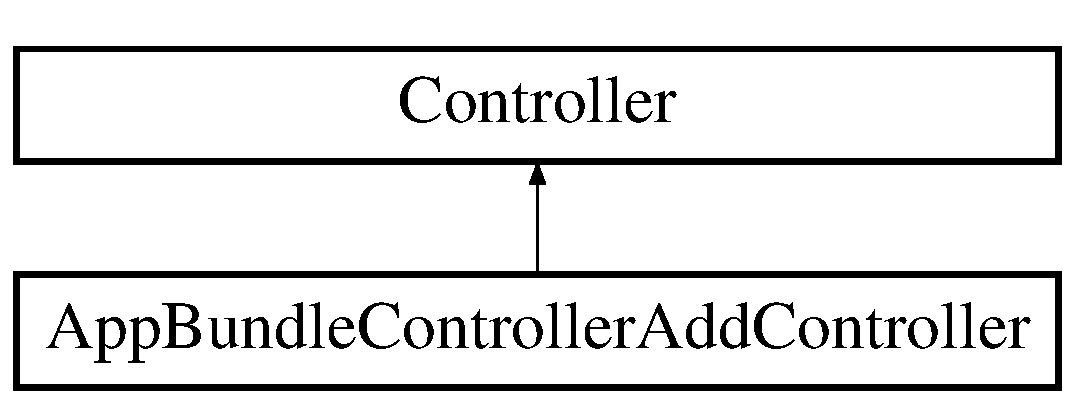
\includegraphics[height=2.000000cm]{class_app_bundle_1_1_controller_1_1_add_controller}
\end{center}
\end{figure}
\subsection*{Public Member Functions}
\begin{DoxyCompactItemize}
\item 
\mbox{\hyperlink{class_app_bundle_1_1_controller_1_1_add_controller_af8ea3325ce33680ab098c54260c63ee8}{add\+Employee\+Action}} (Request \$request)
\end{DoxyCompactItemize}


\subsection{Member Function Documentation}
\mbox{\Hypertarget{class_app_bundle_1_1_controller_1_1_add_controller_af8ea3325ce33680ab098c54260c63ee8}\label{class_app_bundle_1_1_controller_1_1_add_controller_af8ea3325ce33680ab098c54260c63ee8}} 
\index{App\+Bundle\+::\+Controller\+::\+Add\+Controller@{App\+Bundle\+::\+Controller\+::\+Add\+Controller}!add\+Employee\+Action@{add\+Employee\+Action}}
\index{add\+Employee\+Action@{add\+Employee\+Action}!App\+Bundle\+::\+Controller\+::\+Add\+Controller@{App\+Bundle\+::\+Controller\+::\+Add\+Controller}}
\subsubsection{\texorpdfstring{add\+Employee\+Action()}{addEmployeeAction()}}
{\footnotesize\ttfamily App\+Bundle\textbackslash{}\+Controller\textbackslash{}\+Add\+Controller\+::add\+Employee\+Action (\begin{DoxyParamCaption}\item[{Request}]{\$request }\end{DoxyParamCaption})}

(\char`\"{}/add\char`\"{}, name=\char`\"{}add\char`\"{}) (\char`\"{}has\+\_\+role(\textquotesingle{}\+R\+O\+L\+E\+\_\+\+A\+D\+M\+I\+N\textquotesingle{})\char`\"{}) 

The documentation for this class was generated from the following file\+:\begin{DoxyCompactItemize}
\item 
src/\+App\+Bundle/\+Controller/Add\+Controller.\+php\end{DoxyCompactItemize}

\hypertarget{class_app_bundle_1_1_controller_1_1_a_p_i_controller}{}\section{App\+Bundle\textbackslash{}Controller\textbackslash{}A\+P\+I\+Controller Class Reference}
\label{class_app_bundle_1_1_controller_1_1_a_p_i_controller}\index{App\+Bundle\textbackslash{}\+Controller\textbackslash{}\+A\+P\+I\+Controller@{App\+Bundle\textbackslash{}\+Controller\textbackslash{}\+A\+P\+I\+Controller}}
Inheritance diagram for App\+Bundle\textbackslash{}Controller\textbackslash{}A\+P\+I\+Controller\+:\begin{figure}[H]
\begin{center}
\leavevmode
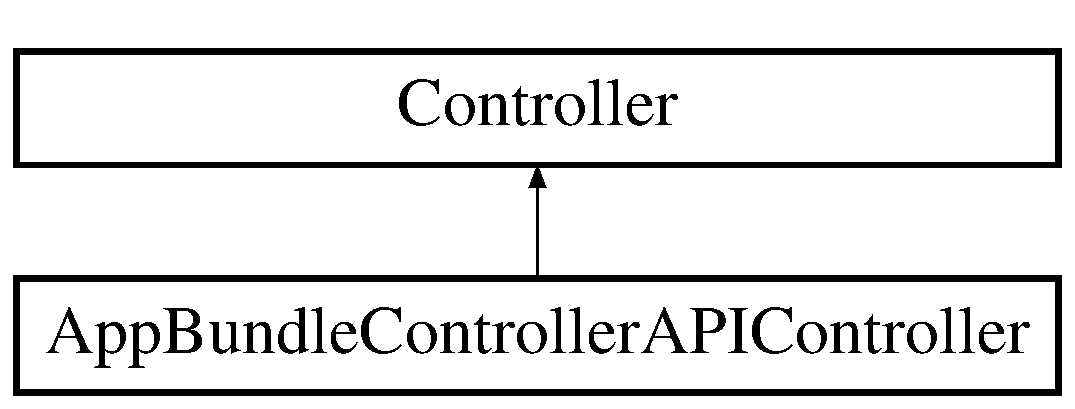
\includegraphics[height=2.000000cm]{class_app_bundle_1_1_controller_1_1_a_p_i_controller}
\end{center}
\end{figure}
\subsection*{Public Member Functions}
\begin{DoxyCompactItemize}
\item 
\mbox{\hyperlink{class_app_bundle_1_1_controller_1_1_a_p_i_controller_a61d1e2704677b4f2b6c469e0ee45c28a}{api\+Action}} ()
\end{DoxyCompactItemize}


\subsection{Member Function Documentation}
\mbox{\Hypertarget{class_app_bundle_1_1_controller_1_1_a_p_i_controller_a61d1e2704677b4f2b6c469e0ee45c28a}\label{class_app_bundle_1_1_controller_1_1_a_p_i_controller_a61d1e2704677b4f2b6c469e0ee45c28a}} 
\index{App\+Bundle\+::\+Controller\+::\+A\+P\+I\+Controller@{App\+Bundle\+::\+Controller\+::\+A\+P\+I\+Controller}!api\+Action@{api\+Action}}
\index{api\+Action@{api\+Action}!App\+Bundle\+::\+Controller\+::\+A\+P\+I\+Controller@{App\+Bundle\+::\+Controller\+::\+A\+P\+I\+Controller}}
\subsubsection{\texorpdfstring{api\+Action()}{apiAction()}}
{\footnotesize\ttfamily App\+Bundle\textbackslash{}\+Controller\textbackslash{}\+A\+P\+I\+Controller\+::api\+Action (\begin{DoxyParamCaption}{ }\end{DoxyParamCaption})}

(\char`\"{}/api\char`\"{}, name=\char`\"{}api\char`\"{}) 

The documentation for this class was generated from the following file\+:\begin{DoxyCompactItemize}
\item 
src/\+App\+Bundle/\+Controller/A\+P\+I\+Controller.\+php\end{DoxyCompactItemize}

\hypertarget{class_app_bundle_1_1_tests_1_1_controller_1_1_a_p_i_controller_test}{}\section{App\+Bundle\textbackslash{}Tests\textbackslash{}Controller\textbackslash{}A\+P\+I\+Controller\+Test Class Reference}
\label{class_app_bundle_1_1_tests_1_1_controller_1_1_a_p_i_controller_test}\index{App\+Bundle\textbackslash{}\+Tests\textbackslash{}\+Controller\textbackslash{}\+A\+P\+I\+Controller\+Test@{App\+Bundle\textbackslash{}\+Tests\textbackslash{}\+Controller\textbackslash{}\+A\+P\+I\+Controller\+Test}}
Inheritance diagram for App\+Bundle\textbackslash{}Tests\textbackslash{}Controller\textbackslash{}A\+P\+I\+Controller\+Test\+:\begin{figure}[H]
\begin{center}
\leavevmode
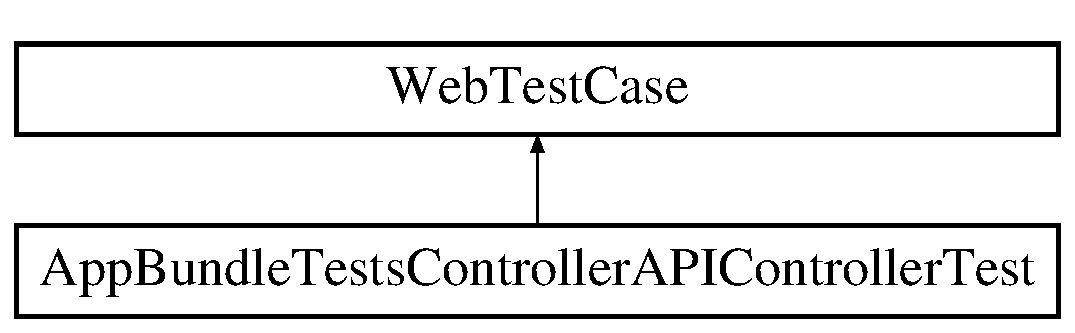
\includegraphics[height=2.000000cm]{class_app_bundle_1_1_tests_1_1_controller_1_1_a_p_i_controller_test}
\end{center}
\end{figure}


The documentation for this class was generated from the following file\+:\begin{DoxyCompactItemize}
\item 
src/\+App\+Bundle/\+Tests/\+Controller/A\+P\+I\+Controller\+Test.\+php\end{DoxyCompactItemize}

\hypertarget{class_app_bundle_1_1_app_bundle}{}\section{App\+Bundle\textbackslash{}App\+Bundle Class Reference}
\label{class_app_bundle_1_1_app_bundle}\index{App\+Bundle\textbackslash{}\+App\+Bundle@{App\+Bundle\textbackslash{}\+App\+Bundle}}
Inheritance diagram for App\+Bundle\textbackslash{}App\+Bundle\+:\begin{figure}[H]
\begin{center}
\leavevmode
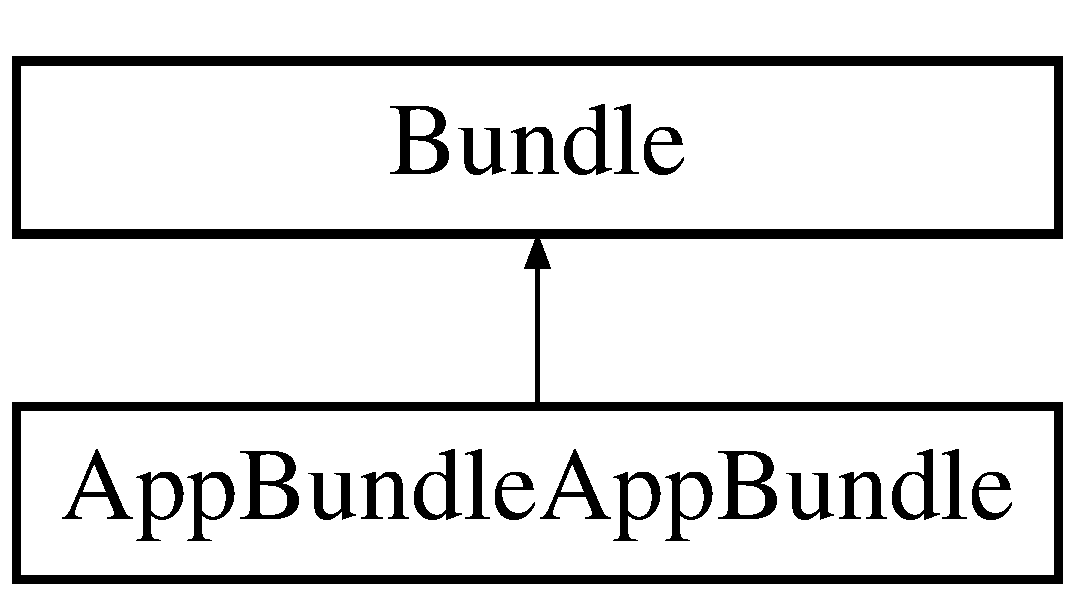
\includegraphics[height=2.000000cm]{class_app_bundle_1_1_app_bundle}
\end{center}
\end{figure}


The documentation for this class was generated from the following file\+:\begin{DoxyCompactItemize}
\item 
src/\+App\+Bundle/App\+Bundle.\+php\end{DoxyCompactItemize}

\hypertarget{class_app_bundle_1_1_controller_1_1_delete_controller}{}\section{App\+Bundle\textbackslash{}Controller\textbackslash{}Delete\+Controller Class Reference}
\label{class_app_bundle_1_1_controller_1_1_delete_controller}\index{App\+Bundle\textbackslash{}\+Controller\textbackslash{}\+Delete\+Controller@{App\+Bundle\textbackslash{}\+Controller\textbackslash{}\+Delete\+Controller}}
Inheritance diagram for App\+Bundle\textbackslash{}Controller\textbackslash{}Delete\+Controller\+:\begin{figure}[H]
\begin{center}
\leavevmode
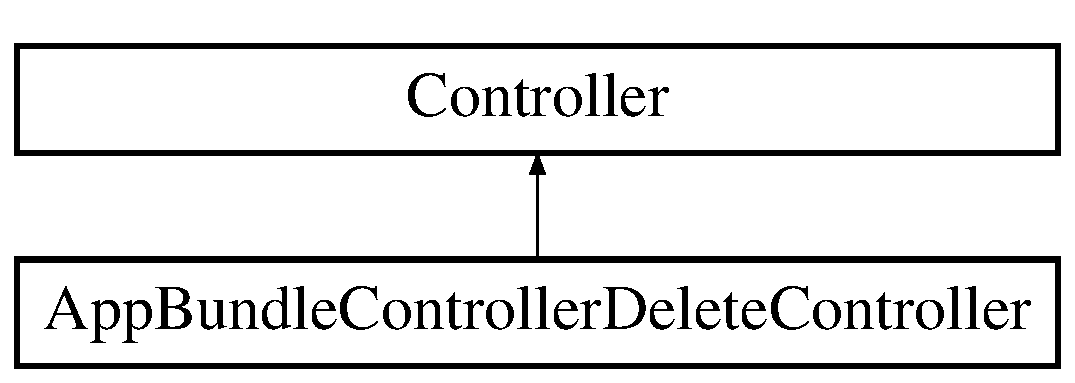
\includegraphics[height=2.000000cm]{class_app_bundle_1_1_controller_1_1_delete_controller}
\end{center}
\end{figure}
\subsection*{Public Member Functions}
\begin{DoxyCompactItemize}
\item 
\mbox{\hyperlink{class_app_bundle_1_1_controller_1_1_delete_controller_accef083f570f50ff66688928c0a37102}{delete\+Employee\+Action}} (Request \$request, \$id)
\end{DoxyCompactItemize}


\subsection{Member Function Documentation}
\mbox{\Hypertarget{class_app_bundle_1_1_controller_1_1_delete_controller_accef083f570f50ff66688928c0a37102}\label{class_app_bundle_1_1_controller_1_1_delete_controller_accef083f570f50ff66688928c0a37102}} 
\index{App\+Bundle\+::\+Controller\+::\+Delete\+Controller@{App\+Bundle\+::\+Controller\+::\+Delete\+Controller}!delete\+Employee\+Action@{delete\+Employee\+Action}}
\index{delete\+Employee\+Action@{delete\+Employee\+Action}!App\+Bundle\+::\+Controller\+::\+Delete\+Controller@{App\+Bundle\+::\+Controller\+::\+Delete\+Controller}}
\subsubsection{\texorpdfstring{delete\+Employee\+Action()}{deleteEmployeeAction()}}
{\footnotesize\ttfamily App\+Bundle\textbackslash{}\+Controller\textbackslash{}\+Delete\+Controller\+::delete\+Employee\+Action (\begin{DoxyParamCaption}\item[{Request}]{\$request,  }\item[{}]{\$id }\end{DoxyParamCaption})}

(\char`\"{}/delete/\{id\}\char`\"{}, name=\char`\"{}delete\char`\"{}) (\char`\"{}has\+\_\+role(\textquotesingle{}\+R\+O\+L\+E\+\_\+\+A\+D\+M\+I\+N\textquotesingle{})\char`\"{}) 

The documentation for this class was generated from the following file\+:\begin{DoxyCompactItemize}
\item 
src/\+App\+Bundle/\+Controller/Delete\+Controller.\+php\end{DoxyCompactItemize}

\hypertarget{class_app_bundle_1_1_tests_1_1_controller_1_1_delete_controller_controller_test}{}\section{App\+Bundle\textbackslash{}Tests\textbackslash{}Controller\textbackslash{}Delete\+Controller\+Controller\+Test Class Reference}
\label{class_app_bundle_1_1_tests_1_1_controller_1_1_delete_controller_controller_test}\index{App\+Bundle\textbackslash{}\+Tests\textbackslash{}\+Controller\textbackslash{}\+Delete\+Controller\+Controller\+Test@{App\+Bundle\textbackslash{}\+Tests\textbackslash{}\+Controller\textbackslash{}\+Delete\+Controller\+Controller\+Test}}
Inheritance diagram for App\+Bundle\textbackslash{}Tests\textbackslash{}Controller\textbackslash{}Delete\+Controller\+Controller\+Test\+:\begin{figure}[H]
\begin{center}
\leavevmode
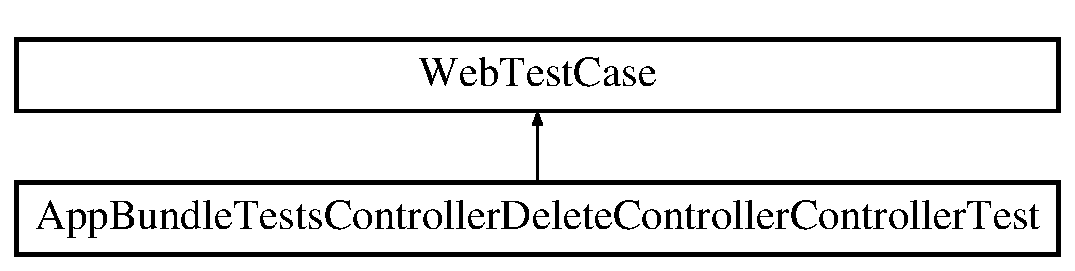
\includegraphics[height=2.000000cm]{class_app_bundle_1_1_tests_1_1_controller_1_1_delete_controller_controller_test}
\end{center}
\end{figure}


The documentation for this class was generated from the following file\+:\begin{DoxyCompactItemize}
\item 
src/\+App\+Bundle/\+Tests/\+Controller/Delete\+Controller\+Controller\+Test.\+php\end{DoxyCompactItemize}

\hypertarget{class_app_bundle_1_1_controller_1_1_details_controller}{}\section{App\+Bundle\textbackslash{}Controller\textbackslash{}Details\+Controller Class Reference}
\label{class_app_bundle_1_1_controller_1_1_details_controller}\index{App\+Bundle\textbackslash{}\+Controller\textbackslash{}\+Details\+Controller@{App\+Bundle\textbackslash{}\+Controller\textbackslash{}\+Details\+Controller}}
Inheritance diagram for App\+Bundle\textbackslash{}Controller\textbackslash{}Details\+Controller\+:\begin{figure}[H]
\begin{center}
\leavevmode
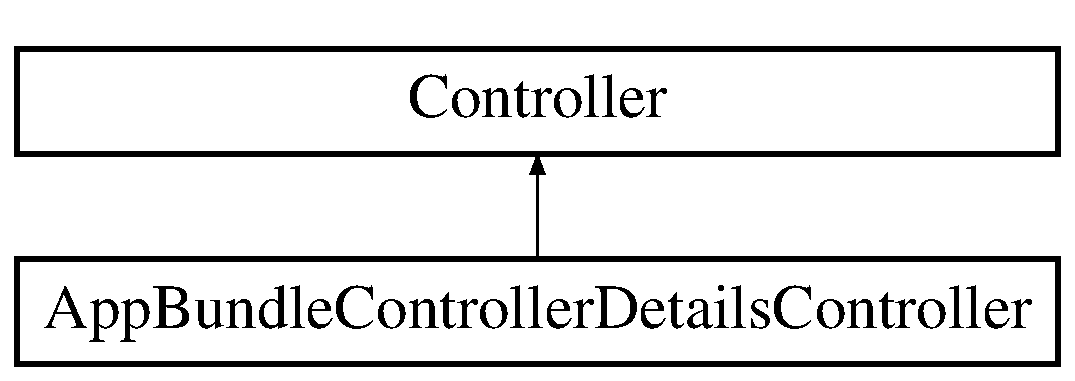
\includegraphics[height=2.000000cm]{class_app_bundle_1_1_controller_1_1_details_controller}
\end{center}
\end{figure}
\subsection*{Public Member Functions}
\begin{DoxyCompactItemize}
\item 
\mbox{\hyperlink{class_app_bundle_1_1_controller_1_1_details_controller_a48005037a3aa333faf089a31ca04f930}{details\+Employee\+Action}} (Request \$request, \$id)
\end{DoxyCompactItemize}


\subsection{Member Function Documentation}
\mbox{\Hypertarget{class_app_bundle_1_1_controller_1_1_details_controller_a48005037a3aa333faf089a31ca04f930}\label{class_app_bundle_1_1_controller_1_1_details_controller_a48005037a3aa333faf089a31ca04f930}} 
\index{App\+Bundle\+::\+Controller\+::\+Details\+Controller@{App\+Bundle\+::\+Controller\+::\+Details\+Controller}!details\+Employee\+Action@{details\+Employee\+Action}}
\index{details\+Employee\+Action@{details\+Employee\+Action}!App\+Bundle\+::\+Controller\+::\+Details\+Controller@{App\+Bundle\+::\+Controller\+::\+Details\+Controller}}
\subsubsection{\texorpdfstring{details\+Employee\+Action()}{detailsEmployeeAction()}}
{\footnotesize\ttfamily App\+Bundle\textbackslash{}\+Controller\textbackslash{}\+Details\+Controller\+::details\+Employee\+Action (\begin{DoxyParamCaption}\item[{Request}]{\$request,  }\item[{}]{\$id }\end{DoxyParamCaption})}

(\char`\"{}/details/\{id\}\char`\"{}, name=\char`\"{}details\char`\"{}) (\char`\"{}has\+\_\+role(\textquotesingle{}\+R\+O\+L\+E\+\_\+\+U\+S\+E\+R\textquotesingle{}) or has\+\_\+role(\textquotesingle{}\+R\+O\+L\+E\+\_\+\+A\+D\+M\+I\+N\textquotesingle{})\char`\"{}) 

The documentation for this class was generated from the following file\+:\begin{DoxyCompactItemize}
\item 
src/\+App\+Bundle/\+Controller/Details\+Controller.\+php\end{DoxyCompactItemize}

\hypertarget{class_app_bundle_1_1_tests_1_1_controller_1_1_details_controller_controller_test}{}\section{App\+Bundle\textbackslash{}Tests\textbackslash{}Controller\textbackslash{}Details\+Controller\+Controller\+Test Class Reference}
\label{class_app_bundle_1_1_tests_1_1_controller_1_1_details_controller_controller_test}\index{App\+Bundle\textbackslash{}\+Tests\textbackslash{}\+Controller\textbackslash{}\+Details\+Controller\+Controller\+Test@{App\+Bundle\textbackslash{}\+Tests\textbackslash{}\+Controller\textbackslash{}\+Details\+Controller\+Controller\+Test}}
Inheritance diagram for App\+Bundle\textbackslash{}Tests\textbackslash{}Controller\textbackslash{}Details\+Controller\+Controller\+Test\+:\begin{figure}[H]
\begin{center}
\leavevmode
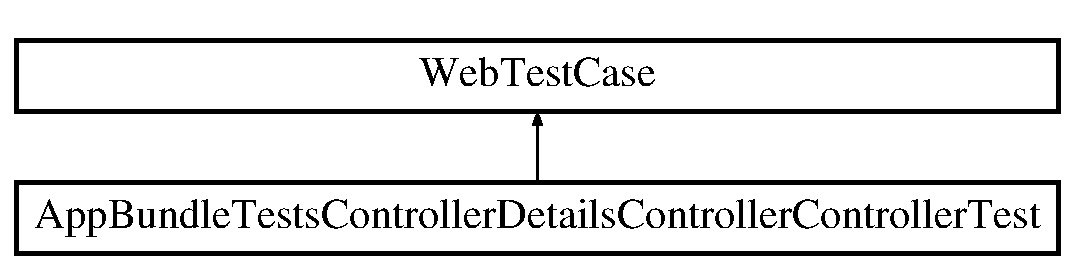
\includegraphics[height=2.000000cm]{class_app_bundle_1_1_tests_1_1_controller_1_1_details_controller_controller_test}
\end{center}
\end{figure}


The documentation for this class was generated from the following file\+:\begin{DoxyCompactItemize}
\item 
src/\+App\+Bundle/\+Tests/\+Controller/Details\+Controller\+Controller\+Test.\+php\end{DoxyCompactItemize}

\hypertarget{class_app_bundle_1_1_controller_1_1_edit_controller}{}\section{App\+Bundle\textbackslash{}Controller\textbackslash{}Edit\+Controller Class Reference}
\label{class_app_bundle_1_1_controller_1_1_edit_controller}\index{App\+Bundle\textbackslash{}\+Controller\textbackslash{}\+Edit\+Controller@{App\+Bundle\textbackslash{}\+Controller\textbackslash{}\+Edit\+Controller}}
Inheritance diagram for App\+Bundle\textbackslash{}Controller\textbackslash{}Edit\+Controller\+:\begin{figure}[H]
\begin{center}
\leavevmode
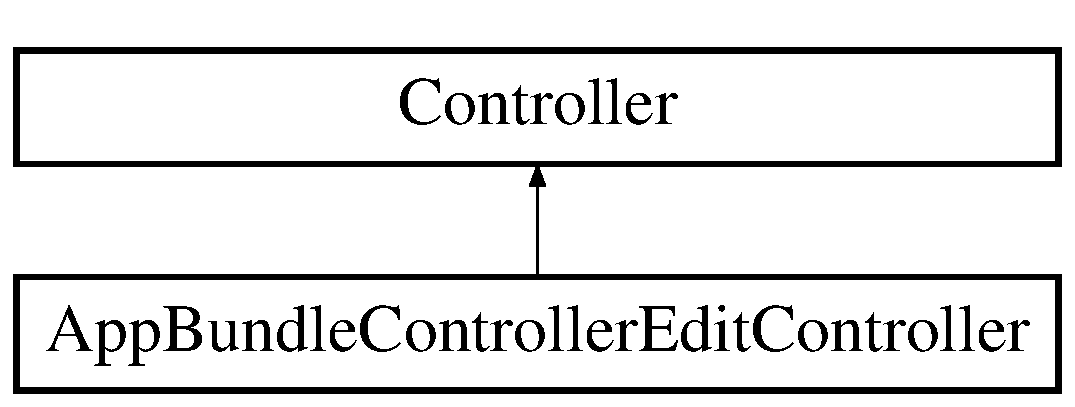
\includegraphics[height=2.000000cm]{class_app_bundle_1_1_controller_1_1_edit_controller}
\end{center}
\end{figure}
\subsection*{Public Member Functions}
\begin{DoxyCompactItemize}
\item 
\mbox{\hyperlink{class_app_bundle_1_1_controller_1_1_edit_controller_a25c5e9d97113d26a4936c897412861cd}{edit\+Employee\+Action}} (Request \$request, \$id)
\end{DoxyCompactItemize}


\subsection{Member Function Documentation}
\mbox{\Hypertarget{class_app_bundle_1_1_controller_1_1_edit_controller_a25c5e9d97113d26a4936c897412861cd}\label{class_app_bundle_1_1_controller_1_1_edit_controller_a25c5e9d97113d26a4936c897412861cd}} 
\index{App\+Bundle\+::\+Controller\+::\+Edit\+Controller@{App\+Bundle\+::\+Controller\+::\+Edit\+Controller}!edit\+Employee\+Action@{edit\+Employee\+Action}}
\index{edit\+Employee\+Action@{edit\+Employee\+Action}!App\+Bundle\+::\+Controller\+::\+Edit\+Controller@{App\+Bundle\+::\+Controller\+::\+Edit\+Controller}}
\subsubsection{\texorpdfstring{edit\+Employee\+Action()}{editEmployeeAction()}}
{\footnotesize\ttfamily App\+Bundle\textbackslash{}\+Controller\textbackslash{}\+Edit\+Controller\+::edit\+Employee\+Action (\begin{DoxyParamCaption}\item[{Request}]{\$request,  }\item[{}]{\$id }\end{DoxyParamCaption})}

(\char`\"{}/edit/\{id\}\char`\"{}, name=\char`\"{}edit\char`\"{}) (\char`\"{}has\+\_\+role(\textquotesingle{}\+R\+O\+L\+E\+\_\+\+A\+D\+M\+I\+N\textquotesingle{})\char`\"{}) 

The documentation for this class was generated from the following file\+:\begin{DoxyCompactItemize}
\item 
src/\+App\+Bundle/\+Controller/Edit\+Controller.\+php\end{DoxyCompactItemize}

\hypertarget{class_app_bundle_1_1_tests_1_1_controller_1_1_edit_controller_controller_test}{}\section{App\+Bundle\textbackslash{}Tests\textbackslash{}Controller\textbackslash{}Edit\+Controller\+Controller\+Test Class Reference}
\label{class_app_bundle_1_1_tests_1_1_controller_1_1_edit_controller_controller_test}\index{App\+Bundle\textbackslash{}\+Tests\textbackslash{}\+Controller\textbackslash{}\+Edit\+Controller\+Controller\+Test@{App\+Bundle\textbackslash{}\+Tests\textbackslash{}\+Controller\textbackslash{}\+Edit\+Controller\+Controller\+Test}}
Inheritance diagram for App\+Bundle\textbackslash{}Tests\textbackslash{}Controller\textbackslash{}Edit\+Controller\+Controller\+Test\+:\begin{figure}[H]
\begin{center}
\leavevmode
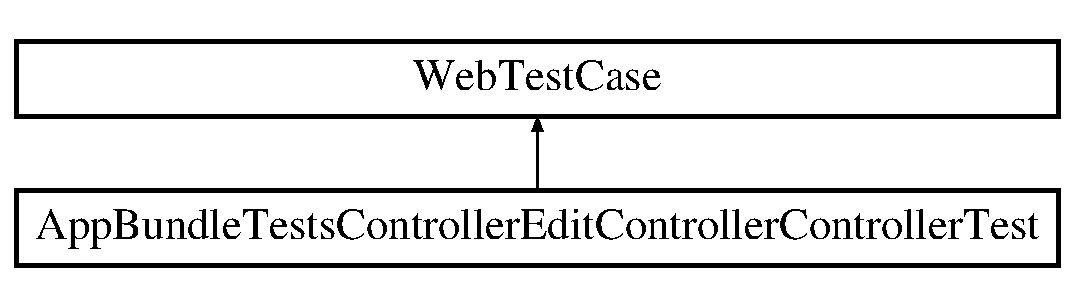
\includegraphics[height=2.000000cm]{class_app_bundle_1_1_tests_1_1_controller_1_1_edit_controller_controller_test}
\end{center}
\end{figure}


The documentation for this class was generated from the following file\+:\begin{DoxyCompactItemize}
\item 
src/\+App\+Bundle/\+Tests/\+Controller/Edit\+Controller\+Controller\+Test.\+php\end{DoxyCompactItemize}

\hypertarget{class_app_bundle_1_1_entity_1_1_employee}{}\section{App\+Bundle\textbackslash{}Entity\textbackslash{}Employee Class Reference}
\label{class_app_bundle_1_1_entity_1_1_employee}\index{App\+Bundle\textbackslash{}\+Entity\textbackslash{}\+Employee@{App\+Bundle\textbackslash{}\+Entity\textbackslash{}\+Employee}}
\subsection*{Public Member Functions}
\begin{DoxyCompactItemize}
\item 
\mbox{\hyperlink{class_app_bundle_1_1_entity_1_1_employee_a8a71f05623bc36531c265d4687907530}{get\+Id}} ()
\item 
\mbox{\hyperlink{class_app_bundle_1_1_entity_1_1_employee_a26c8846a99373bcfc48e48ba828ed638}{set\+Firstname}} (\$firstname)
\item 
\mbox{\hyperlink{class_app_bundle_1_1_entity_1_1_employee_a113700e4ca507530c4d36f9dd9b3e1f8}{get\+Firstname}} ()
\item 
\mbox{\hyperlink{class_app_bundle_1_1_entity_1_1_employee_a2df5450a8b6fa806ab2eb0fca83c8adb}{set\+Lastname}} (\$lastname)
\item 
\mbox{\hyperlink{class_app_bundle_1_1_entity_1_1_employee_a0531339740880fea55260af8a4d47628}{get\+Lastname}} ()
\item 
\mbox{\hyperlink{class_app_bundle_1_1_entity_1_1_employee_a1eaa0241464490a7b907de2b86ccee0e}{set\+Age}} (\$age)
\item 
\mbox{\hyperlink{class_app_bundle_1_1_entity_1_1_employee_aa2f51fb4f112bb2b96f58d4d13f2d556}{get\+Age}} ()
\item 
\mbox{\hyperlink{class_app_bundle_1_1_entity_1_1_employee_a65a7565c426fdea00b46bb5453f75465}{set\+Job}} (\$job)
\item 
\mbox{\hyperlink{class_app_bundle_1_1_entity_1_1_employee_ab3315de55e8e5285ec30ef7e21db7590}{get\+Job}} ()
\item 
\mbox{\hyperlink{class_app_bundle_1_1_entity_1_1_employee_a32ca49cdd8a94c7cb916977a3ce5fa71}{set\+Phone}} (\$phone)
\item 
\mbox{\hyperlink{class_app_bundle_1_1_entity_1_1_employee_a7aae3372e50769995ac7ac3f4a5c7ac4}{get\+Phone}} ()
\item 
\mbox{\hyperlink{class_app_bundle_1_1_entity_1_1_employee_abc7b0c40463197bd32bc452e9ffe4407}{set\+Environment}} (\mbox{\hyperlink{class_app_bundle_1_1_entity_1_1_environment}{Environment}} \$environment)
\item 
\mbox{\hyperlink{class_app_bundle_1_1_entity_1_1_employee_a1eefb3ea4030d24b24ad529f4a20de21}{Get\+Environment}} ()
\item 
\mbox{\Hypertarget{class_app_bundle_1_1_entity_1_1_employee_a8dbb03f672dce72b8a92d5ac77e27286}\label{class_app_bundle_1_1_entity_1_1_employee_a8dbb03f672dce72b8a92d5ac77e27286}} 
{\bfseries add\+Skills} (\mbox{\hyperlink{class_app_bundle_1_1_entity_1_1_skill}{Skill}} \$skill)
\item 
\mbox{\Hypertarget{class_app_bundle_1_1_entity_1_1_employee_a68fb017db13b94a968d43d1b636805d2}\label{class_app_bundle_1_1_entity_1_1_employee_a68fb017db13b94a968d43d1b636805d2}} 
{\bfseries get\+Skills} ()
\item 
\mbox{\hyperlink{class_app_bundle_1_1_entity_1_1_employee_afc80996e5115964f45fd60d9d55630fb}{add\+Skill}} (\textbackslash{}App\+Bundle\textbackslash{}\+Entity\textbackslash{}\+Skills \$skill)
\item 
\mbox{\hyperlink{class_app_bundle_1_1_entity_1_1_employee_a69717b66303d554ad4c4297c147ad01d}{remove\+Skill}} (\textbackslash{}App\+Bundle\textbackslash{}\+Entity\textbackslash{}\+Skills \$skill)
\end{DoxyCompactItemize}
\subsection*{Public Attributes}
\begin{DoxyCompactItemize}
\item 
\mbox{\hyperlink{class_app_bundle_1_1_entity_1_1_employee_ac121b7a30226c432e050d3d3c611cb7d}{\$skills}}
\end{DoxyCompactItemize}


\subsection{Detailed Description}
\mbox{\hyperlink{class_app_bundle_1_1_entity_1_1_employee}{Employee}}

(name=\char`\"{}employee\char`\"{}) (repository\+Class=\char`\"{}\+App\+Bundle\textbackslash{}\+Repository\textbackslash{}\+Employee\+Repository\char`\"{}) 

\subsection{Member Function Documentation}
\mbox{\Hypertarget{class_app_bundle_1_1_entity_1_1_employee_afc80996e5115964f45fd60d9d55630fb}\label{class_app_bundle_1_1_entity_1_1_employee_afc80996e5115964f45fd60d9d55630fb}} 
\index{App\+Bundle\+::\+Entity\+::\+Employee@{App\+Bundle\+::\+Entity\+::\+Employee}!add\+Skill@{add\+Skill}}
\index{add\+Skill@{add\+Skill}!App\+Bundle\+::\+Entity\+::\+Employee@{App\+Bundle\+::\+Entity\+::\+Employee}}
\subsubsection{\texorpdfstring{add\+Skill()}{addSkill()}}
{\footnotesize\ttfamily App\+Bundle\textbackslash{}\+Entity\textbackslash{}\+Employee\+::add\+Skill (\begin{DoxyParamCaption}\item[{\textbackslash{}App\+Bundle\textbackslash{}\+Entity\textbackslash{}\+Skills}]{\$skill }\end{DoxyParamCaption})}

Add skill


\begin{DoxyParams}[1]{Parameters}
\textbackslash{}\+App\+Bundle\textbackslash{}\+Entity\textbackslash{}\+Skills & {\em \$skill} & \\
\hline
\end{DoxyParams}
\begin{DoxyReturn}{Returns}
\mbox{\hyperlink{class_app_bundle_1_1_entity_1_1_employee}{Employee}} 
\end{DoxyReturn}
\mbox{\Hypertarget{class_app_bundle_1_1_entity_1_1_employee_aa2f51fb4f112bb2b96f58d4d13f2d556}\label{class_app_bundle_1_1_entity_1_1_employee_aa2f51fb4f112bb2b96f58d4d13f2d556}} 
\index{App\+Bundle\+::\+Entity\+::\+Employee@{App\+Bundle\+::\+Entity\+::\+Employee}!get\+Age@{get\+Age}}
\index{get\+Age@{get\+Age}!App\+Bundle\+::\+Entity\+::\+Employee@{App\+Bundle\+::\+Entity\+::\+Employee}}
\subsubsection{\texorpdfstring{get\+Age()}{getAge()}}
{\footnotesize\ttfamily App\+Bundle\textbackslash{}\+Entity\textbackslash{}\+Employee\+::get\+Age (\begin{DoxyParamCaption}{ }\end{DoxyParamCaption})}

Get age

\begin{DoxyReturn}{Returns}
int 
\end{DoxyReturn}
\mbox{\Hypertarget{class_app_bundle_1_1_entity_1_1_employee_a1eefb3ea4030d24b24ad529f4a20de21}\label{class_app_bundle_1_1_entity_1_1_employee_a1eefb3ea4030d24b24ad529f4a20de21}} 
\index{App\+Bundle\+::\+Entity\+::\+Employee@{App\+Bundle\+::\+Entity\+::\+Employee}!Get\+Environment@{Get\+Environment}}
\index{Get\+Environment@{Get\+Environment}!App\+Bundle\+::\+Entity\+::\+Employee@{App\+Bundle\+::\+Entity\+::\+Employee}}
\subsubsection{\texorpdfstring{Get\+Environment()}{GetEnvironment()}}
{\footnotesize\ttfamily App\+Bundle\textbackslash{}\+Entity\textbackslash{}\+Employee\+::\+Get\+Environment (\begin{DoxyParamCaption}{ }\end{DoxyParamCaption})}

Get environment

\begin{DoxyReturn}{Returns}
environment 
\end{DoxyReturn}
\mbox{\Hypertarget{class_app_bundle_1_1_entity_1_1_employee_a113700e4ca507530c4d36f9dd9b3e1f8}\label{class_app_bundle_1_1_entity_1_1_employee_a113700e4ca507530c4d36f9dd9b3e1f8}} 
\index{App\+Bundle\+::\+Entity\+::\+Employee@{App\+Bundle\+::\+Entity\+::\+Employee}!get\+Firstname@{get\+Firstname}}
\index{get\+Firstname@{get\+Firstname}!App\+Bundle\+::\+Entity\+::\+Employee@{App\+Bundle\+::\+Entity\+::\+Employee}}
\subsubsection{\texorpdfstring{get\+Firstname()}{getFirstname()}}
{\footnotesize\ttfamily App\+Bundle\textbackslash{}\+Entity\textbackslash{}\+Employee\+::get\+Firstname (\begin{DoxyParamCaption}{ }\end{DoxyParamCaption})}

Get firstname

\begin{DoxyReturn}{Returns}
string 
\end{DoxyReturn}
\mbox{\Hypertarget{class_app_bundle_1_1_entity_1_1_employee_a8a71f05623bc36531c265d4687907530}\label{class_app_bundle_1_1_entity_1_1_employee_a8a71f05623bc36531c265d4687907530}} 
\index{App\+Bundle\+::\+Entity\+::\+Employee@{App\+Bundle\+::\+Entity\+::\+Employee}!get\+Id@{get\+Id}}
\index{get\+Id@{get\+Id}!App\+Bundle\+::\+Entity\+::\+Employee@{App\+Bundle\+::\+Entity\+::\+Employee}}
\subsubsection{\texorpdfstring{get\+Id()}{getId()}}
{\footnotesize\ttfamily App\+Bundle\textbackslash{}\+Entity\textbackslash{}\+Employee\+::get\+Id (\begin{DoxyParamCaption}{ }\end{DoxyParamCaption})}

Get id

\begin{DoxyReturn}{Returns}
int 
\end{DoxyReturn}
\mbox{\Hypertarget{class_app_bundle_1_1_entity_1_1_employee_ab3315de55e8e5285ec30ef7e21db7590}\label{class_app_bundle_1_1_entity_1_1_employee_ab3315de55e8e5285ec30ef7e21db7590}} 
\index{App\+Bundle\+::\+Entity\+::\+Employee@{App\+Bundle\+::\+Entity\+::\+Employee}!get\+Job@{get\+Job}}
\index{get\+Job@{get\+Job}!App\+Bundle\+::\+Entity\+::\+Employee@{App\+Bundle\+::\+Entity\+::\+Employee}}
\subsubsection{\texorpdfstring{get\+Job()}{getJob()}}
{\footnotesize\ttfamily App\+Bundle\textbackslash{}\+Entity\textbackslash{}\+Employee\+::get\+Job (\begin{DoxyParamCaption}{ }\end{DoxyParamCaption})}

Get job

\begin{DoxyReturn}{Returns}
string 
\end{DoxyReturn}
\mbox{\Hypertarget{class_app_bundle_1_1_entity_1_1_employee_a0531339740880fea55260af8a4d47628}\label{class_app_bundle_1_1_entity_1_1_employee_a0531339740880fea55260af8a4d47628}} 
\index{App\+Bundle\+::\+Entity\+::\+Employee@{App\+Bundle\+::\+Entity\+::\+Employee}!get\+Lastname@{get\+Lastname}}
\index{get\+Lastname@{get\+Lastname}!App\+Bundle\+::\+Entity\+::\+Employee@{App\+Bundle\+::\+Entity\+::\+Employee}}
\subsubsection{\texorpdfstring{get\+Lastname()}{getLastname()}}
{\footnotesize\ttfamily App\+Bundle\textbackslash{}\+Entity\textbackslash{}\+Employee\+::get\+Lastname (\begin{DoxyParamCaption}{ }\end{DoxyParamCaption})}

Get lastname

\begin{DoxyReturn}{Returns}
string 
\end{DoxyReturn}
\mbox{\Hypertarget{class_app_bundle_1_1_entity_1_1_employee_a7aae3372e50769995ac7ac3f4a5c7ac4}\label{class_app_bundle_1_1_entity_1_1_employee_a7aae3372e50769995ac7ac3f4a5c7ac4}} 
\index{App\+Bundle\+::\+Entity\+::\+Employee@{App\+Bundle\+::\+Entity\+::\+Employee}!get\+Phone@{get\+Phone}}
\index{get\+Phone@{get\+Phone}!App\+Bundle\+::\+Entity\+::\+Employee@{App\+Bundle\+::\+Entity\+::\+Employee}}
\subsubsection{\texorpdfstring{get\+Phone()}{getPhone()}}
{\footnotesize\ttfamily App\+Bundle\textbackslash{}\+Entity\textbackslash{}\+Employee\+::get\+Phone (\begin{DoxyParamCaption}{ }\end{DoxyParamCaption})}

Get phone

\begin{DoxyReturn}{Returns}
string 
\end{DoxyReturn}
\mbox{\Hypertarget{class_app_bundle_1_1_entity_1_1_employee_a69717b66303d554ad4c4297c147ad01d}\label{class_app_bundle_1_1_entity_1_1_employee_a69717b66303d554ad4c4297c147ad01d}} 
\index{App\+Bundle\+::\+Entity\+::\+Employee@{App\+Bundle\+::\+Entity\+::\+Employee}!remove\+Skill@{remove\+Skill}}
\index{remove\+Skill@{remove\+Skill}!App\+Bundle\+::\+Entity\+::\+Employee@{App\+Bundle\+::\+Entity\+::\+Employee}}
\subsubsection{\texorpdfstring{remove\+Skill()}{removeSkill()}}
{\footnotesize\ttfamily App\+Bundle\textbackslash{}\+Entity\textbackslash{}\+Employee\+::remove\+Skill (\begin{DoxyParamCaption}\item[{\textbackslash{}App\+Bundle\textbackslash{}\+Entity\textbackslash{}\+Skills}]{\$skill }\end{DoxyParamCaption})}

Remove skill


\begin{DoxyParams}[1]{Parameters}
\textbackslash{}\+App\+Bundle\textbackslash{}\+Entity\textbackslash{}\+Skills & {\em \$skill} & \\
\hline
\end{DoxyParams}
\mbox{\Hypertarget{class_app_bundle_1_1_entity_1_1_employee_a1eaa0241464490a7b907de2b86ccee0e}\label{class_app_bundle_1_1_entity_1_1_employee_a1eaa0241464490a7b907de2b86ccee0e}} 
\index{App\+Bundle\+::\+Entity\+::\+Employee@{App\+Bundle\+::\+Entity\+::\+Employee}!set\+Age@{set\+Age}}
\index{set\+Age@{set\+Age}!App\+Bundle\+::\+Entity\+::\+Employee@{App\+Bundle\+::\+Entity\+::\+Employee}}
\subsubsection{\texorpdfstring{set\+Age()}{setAge()}}
{\footnotesize\ttfamily App\+Bundle\textbackslash{}\+Entity\textbackslash{}\+Employee\+::set\+Age (\begin{DoxyParamCaption}\item[{}]{\$age }\end{DoxyParamCaption})}

Set age


\begin{DoxyParams}[1]{Parameters}
integer & {\em \$age} & \\
\hline
\end{DoxyParams}
\begin{DoxyReturn}{Returns}
\mbox{\hyperlink{class_app_bundle_1_1_entity_1_1_employee}{Employee}} 
\end{DoxyReturn}
\mbox{\Hypertarget{class_app_bundle_1_1_entity_1_1_employee_abc7b0c40463197bd32bc452e9ffe4407}\label{class_app_bundle_1_1_entity_1_1_employee_abc7b0c40463197bd32bc452e9ffe4407}} 
\index{App\+Bundle\+::\+Entity\+::\+Employee@{App\+Bundle\+::\+Entity\+::\+Employee}!set\+Environment@{set\+Environment}}
\index{set\+Environment@{set\+Environment}!App\+Bundle\+::\+Entity\+::\+Employee@{App\+Bundle\+::\+Entity\+::\+Employee}}
\subsubsection{\texorpdfstring{set\+Environment()}{setEnvironment()}}
{\footnotesize\ttfamily App\+Bundle\textbackslash{}\+Entity\textbackslash{}\+Employee\+::set\+Environment (\begin{DoxyParamCaption}\item[{\mbox{\hyperlink{class_app_bundle_1_1_entity_1_1_environment}{Environment}}}]{\$environment }\end{DoxyParamCaption})}

Set environment


\begin{DoxyParams}[1]{Parameters}
\mbox{\hyperlink{class_app_bundle_1_1_entity_1_1_environment}{Environment}} & {\em \$environment} & \\
\hline
\end{DoxyParams}
\begin{DoxyReturn}{Returns}
\mbox{\hyperlink{class_app_bundle_1_1_entity_1_1_employee}{Employee}} 
\end{DoxyReturn}
\mbox{\Hypertarget{class_app_bundle_1_1_entity_1_1_employee_a26c8846a99373bcfc48e48ba828ed638}\label{class_app_bundle_1_1_entity_1_1_employee_a26c8846a99373bcfc48e48ba828ed638}} 
\index{App\+Bundle\+::\+Entity\+::\+Employee@{App\+Bundle\+::\+Entity\+::\+Employee}!set\+Firstname@{set\+Firstname}}
\index{set\+Firstname@{set\+Firstname}!App\+Bundle\+::\+Entity\+::\+Employee@{App\+Bundle\+::\+Entity\+::\+Employee}}
\subsubsection{\texorpdfstring{set\+Firstname()}{setFirstname()}}
{\footnotesize\ttfamily App\+Bundle\textbackslash{}\+Entity\textbackslash{}\+Employee\+::set\+Firstname (\begin{DoxyParamCaption}\item[{}]{\$firstname }\end{DoxyParamCaption})}

Set firstname


\begin{DoxyParams}[1]{Parameters}
string & {\em \$firstname} & \\
\hline
\end{DoxyParams}
\begin{DoxyReturn}{Returns}
\mbox{\hyperlink{class_app_bundle_1_1_entity_1_1_employee}{Employee}} 
\end{DoxyReturn}
\mbox{\Hypertarget{class_app_bundle_1_1_entity_1_1_employee_a65a7565c426fdea00b46bb5453f75465}\label{class_app_bundle_1_1_entity_1_1_employee_a65a7565c426fdea00b46bb5453f75465}} 
\index{App\+Bundle\+::\+Entity\+::\+Employee@{App\+Bundle\+::\+Entity\+::\+Employee}!set\+Job@{set\+Job}}
\index{set\+Job@{set\+Job}!App\+Bundle\+::\+Entity\+::\+Employee@{App\+Bundle\+::\+Entity\+::\+Employee}}
\subsubsection{\texorpdfstring{set\+Job()}{setJob()}}
{\footnotesize\ttfamily App\+Bundle\textbackslash{}\+Entity\textbackslash{}\+Employee\+::set\+Job (\begin{DoxyParamCaption}\item[{}]{\$job }\end{DoxyParamCaption})}

Set job


\begin{DoxyParams}[1]{Parameters}
string & {\em \$job} & \\
\hline
\end{DoxyParams}
\begin{DoxyReturn}{Returns}
\mbox{\hyperlink{class_app_bundle_1_1_entity_1_1_employee}{Employee}} 
\end{DoxyReturn}
\mbox{\Hypertarget{class_app_bundle_1_1_entity_1_1_employee_a2df5450a8b6fa806ab2eb0fca83c8adb}\label{class_app_bundle_1_1_entity_1_1_employee_a2df5450a8b6fa806ab2eb0fca83c8adb}} 
\index{App\+Bundle\+::\+Entity\+::\+Employee@{App\+Bundle\+::\+Entity\+::\+Employee}!set\+Lastname@{set\+Lastname}}
\index{set\+Lastname@{set\+Lastname}!App\+Bundle\+::\+Entity\+::\+Employee@{App\+Bundle\+::\+Entity\+::\+Employee}}
\subsubsection{\texorpdfstring{set\+Lastname()}{setLastname()}}
{\footnotesize\ttfamily App\+Bundle\textbackslash{}\+Entity\textbackslash{}\+Employee\+::set\+Lastname (\begin{DoxyParamCaption}\item[{}]{\$lastname }\end{DoxyParamCaption})}

Set lastname


\begin{DoxyParams}[1]{Parameters}
string & {\em \$lastname} & \\
\hline
\end{DoxyParams}
\begin{DoxyReturn}{Returns}
\mbox{\hyperlink{class_app_bundle_1_1_entity_1_1_employee}{Employee}} 
\end{DoxyReturn}
\mbox{\Hypertarget{class_app_bundle_1_1_entity_1_1_employee_a32ca49cdd8a94c7cb916977a3ce5fa71}\label{class_app_bundle_1_1_entity_1_1_employee_a32ca49cdd8a94c7cb916977a3ce5fa71}} 
\index{App\+Bundle\+::\+Entity\+::\+Employee@{App\+Bundle\+::\+Entity\+::\+Employee}!set\+Phone@{set\+Phone}}
\index{set\+Phone@{set\+Phone}!App\+Bundle\+::\+Entity\+::\+Employee@{App\+Bundle\+::\+Entity\+::\+Employee}}
\subsubsection{\texorpdfstring{set\+Phone()}{setPhone()}}
{\footnotesize\ttfamily App\+Bundle\textbackslash{}\+Entity\textbackslash{}\+Employee\+::set\+Phone (\begin{DoxyParamCaption}\item[{}]{\$phone }\end{DoxyParamCaption})}

Set phone


\begin{DoxyParams}[1]{Parameters}
string & {\em \$phone} & \\
\hline
\end{DoxyParams}
\begin{DoxyReturn}{Returns}
\mbox{\hyperlink{class_app_bundle_1_1_entity_1_1_employee}{Employee}} 
\end{DoxyReturn}


\subsection{Member Data Documentation}
\mbox{\Hypertarget{class_app_bundle_1_1_entity_1_1_employee_ac121b7a30226c432e050d3d3c611cb7d}\label{class_app_bundle_1_1_entity_1_1_employee_ac121b7a30226c432e050d3d3c611cb7d}} 
\index{App\+Bundle\+::\+Entity\+::\+Employee@{App\+Bundle\+::\+Entity\+::\+Employee}!\$skills@{\$skills}}
\index{\$skills@{\$skills}!App\+Bundle\+::\+Entity\+::\+Employee@{App\+Bundle\+::\+Entity\+::\+Employee}}
\subsubsection{\texorpdfstring{\$skills}{$skills}}
{\footnotesize\ttfamily App\+Bundle\textbackslash{}\+Entity\textbackslash{}\+Employee\+::\$skills}

(target\+Entity=\char`\"{}\+Skill\char`\"{}, mapped\+By=\char`\"{}employee\char`\"{}) 

The documentation for this class was generated from the following file\+:\begin{DoxyCompactItemize}
\item 
src/\+App\+Bundle/\+Entity/Employee.\+php\end{DoxyCompactItemize}

\hypertarget{class_app_bundle_1_1_controller_1_1_employee_controller}{}\section{App\+Bundle\textbackslash{}Controller\textbackslash{}Employee\+Controller Class Reference}
\label{class_app_bundle_1_1_controller_1_1_employee_controller}\index{App\+Bundle\textbackslash{}\+Controller\textbackslash{}\+Employee\+Controller@{App\+Bundle\textbackslash{}\+Controller\textbackslash{}\+Employee\+Controller}}
Inheritance diagram for App\+Bundle\textbackslash{}Controller\textbackslash{}Employee\+Controller\+:\begin{figure}[H]
\begin{center}
\leavevmode
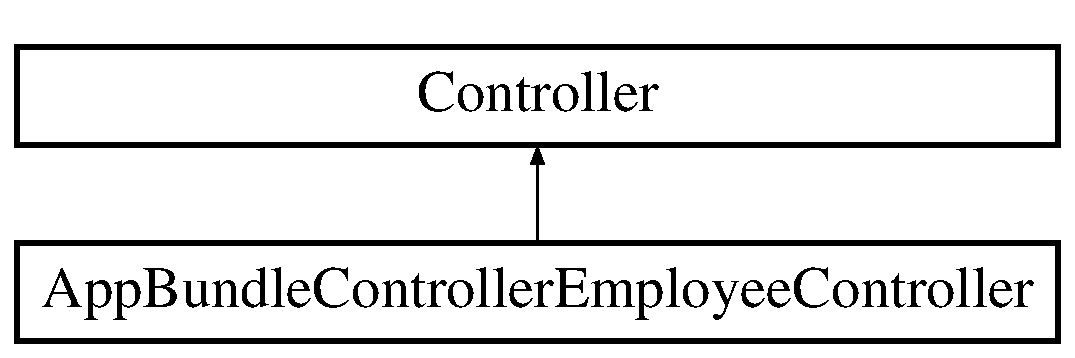
\includegraphics[height=2.000000cm]{class_app_bundle_1_1_controller_1_1_employee_controller}
\end{center}
\end{figure}
\subsection*{Public Member Functions}
\begin{DoxyCompactItemize}
\item 
\mbox{\hyperlink{class_app_bundle_1_1_controller_1_1_employee_controller_af8d48d3c6654baacd1505b289e64070a}{index\+Action}} ()
\item 
\mbox{\hyperlink{class_app_bundle_1_1_controller_1_1_employee_controller_a7392ff83d0857c8e8ee5e3a8707ce4cf}{show\+Action}} (\mbox{\hyperlink{class_app_bundle_1_1_entity_1_1_employee}{Employee}} \$employee)
\end{DoxyCompactItemize}


\subsection{Detailed Description}
Employee controller.

(\char`\"{}employee\char`\"{}) 

\subsection{Member Function Documentation}
\mbox{\Hypertarget{class_app_bundle_1_1_controller_1_1_employee_controller_af8d48d3c6654baacd1505b289e64070a}\label{class_app_bundle_1_1_controller_1_1_employee_controller_af8d48d3c6654baacd1505b289e64070a}} 
\index{App\+Bundle\+::\+Controller\+::\+Employee\+Controller@{App\+Bundle\+::\+Controller\+::\+Employee\+Controller}!index\+Action@{index\+Action}}
\index{index\+Action@{index\+Action}!App\+Bundle\+::\+Controller\+::\+Employee\+Controller@{App\+Bundle\+::\+Controller\+::\+Employee\+Controller}}
\subsubsection{\texorpdfstring{index\+Action()}{indexAction()}}
{\footnotesize\ttfamily App\+Bundle\textbackslash{}\+Controller\textbackslash{}\+Employee\+Controller\+::index\+Action (\begin{DoxyParamCaption}{ }\end{DoxyParamCaption})}

Lists all employee entities.

(\char`\"{}/\char`\"{}, name=\char`\"{}employee\+\_\+index\char`\"{}) (\char`\"{}\+G\+E\+T\char`\"{}) (\char`\"{}has\+\_\+role(\textquotesingle{}\+R\+O\+L\+E\+\_\+\+U\+S\+E\+R\textquotesingle{})\char`\"{}) \mbox{\Hypertarget{class_app_bundle_1_1_controller_1_1_employee_controller_a7392ff83d0857c8e8ee5e3a8707ce4cf}\label{class_app_bundle_1_1_controller_1_1_employee_controller_a7392ff83d0857c8e8ee5e3a8707ce4cf}} 
\index{App\+Bundle\+::\+Controller\+::\+Employee\+Controller@{App\+Bundle\+::\+Controller\+::\+Employee\+Controller}!show\+Action@{show\+Action}}
\index{show\+Action@{show\+Action}!App\+Bundle\+::\+Controller\+::\+Employee\+Controller@{App\+Bundle\+::\+Controller\+::\+Employee\+Controller}}
\subsubsection{\texorpdfstring{show\+Action()}{showAction()}}
{\footnotesize\ttfamily App\+Bundle\textbackslash{}\+Controller\textbackslash{}\+Employee\+Controller\+::show\+Action (\begin{DoxyParamCaption}\item[{\mbox{\hyperlink{class_app_bundle_1_1_entity_1_1_employee}{Employee}}}]{\$employee }\end{DoxyParamCaption})}

Finds and displays a employee entity.

(\char`\"{}/\{id\}\char`\"{}, name=\char`\"{}employee\+\_\+show\char`\"{}) (\char`\"{}\+G\+E\+T\char`\"{}) (\char`\"{}has\+\_\+role(\textquotesingle{}\+R\+O\+L\+E\+\_\+\+U\+S\+E\+R\textquotesingle{})\char`\"{}) 

The documentation for this class was generated from the following file\+:\begin{DoxyCompactItemize}
\item 
src/\+App\+Bundle/\+Controller/Employee\+Controller.\+php\end{DoxyCompactItemize}

\hypertarget{class_app_bundle_1_1_tests_1_1_controller_1_1_employee_controller_test}{}\section{App\+Bundle\textbackslash{}Tests\textbackslash{}Controller\textbackslash{}Employee\+Controller\+Test Class Reference}
\label{class_app_bundle_1_1_tests_1_1_controller_1_1_employee_controller_test}\index{App\+Bundle\textbackslash{}\+Tests\textbackslash{}\+Controller\textbackslash{}\+Employee\+Controller\+Test@{App\+Bundle\textbackslash{}\+Tests\textbackslash{}\+Controller\textbackslash{}\+Employee\+Controller\+Test}}
Inheritance diagram for App\+Bundle\textbackslash{}Tests\textbackslash{}Controller\textbackslash{}Employee\+Controller\+Test\+:\begin{figure}[H]
\begin{center}
\leavevmode
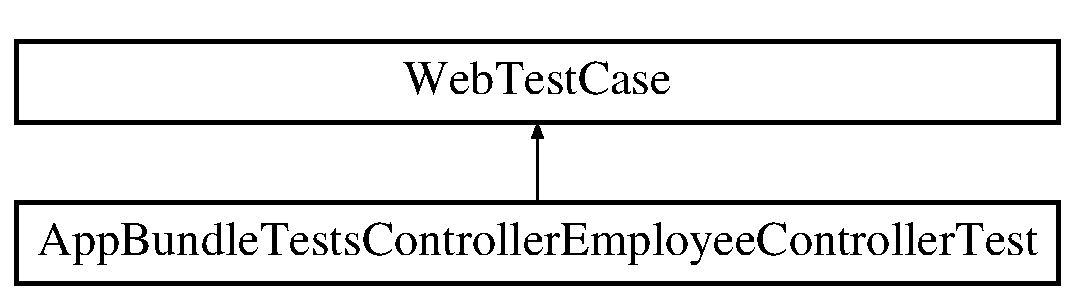
\includegraphics[height=2.000000cm]{class_app_bundle_1_1_tests_1_1_controller_1_1_employee_controller_test}
\end{center}
\end{figure}


The documentation for this class was generated from the following file\+:\begin{DoxyCompactItemize}
\item 
src/\+App\+Bundle/\+Tests/\+Controller/Employee\+Controller\+Test.\+php\end{DoxyCompactItemize}

\hypertarget{class_app_bundle_1_1_repository_1_1_employee_repository}{}\section{App\+Bundle\textbackslash{}Repository\textbackslash{}Employee\+Repository Class Reference}
\label{class_app_bundle_1_1_repository_1_1_employee_repository}\index{App\+Bundle\textbackslash{}\+Repository\textbackslash{}\+Employee\+Repository@{App\+Bundle\textbackslash{}\+Repository\textbackslash{}\+Employee\+Repository}}
Inheritance diagram for App\+Bundle\textbackslash{}Repository\textbackslash{}Employee\+Repository\+:\begin{figure}[H]
\begin{center}
\leavevmode
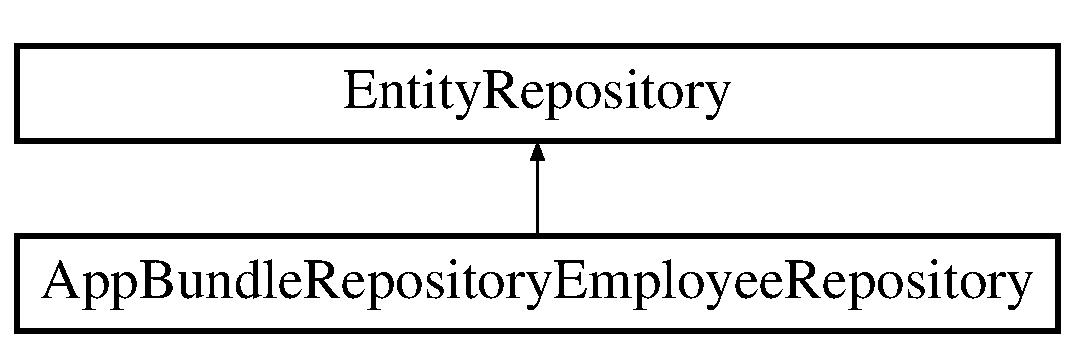
\includegraphics[height=2.000000cm]{class_app_bundle_1_1_repository_1_1_employee_repository}
\end{center}
\end{figure}


\subsection{Detailed Description}
\mbox{\hyperlink{class_app_bundle_1_1_repository_1_1_employee_repository}{Employee\+Repository}}

This class was generated by the Doctrine O\+RM. Add your own custom repository methods below. 

The documentation for this class was generated from the following file\+:\begin{DoxyCompactItemize}
\item 
src/\+App\+Bundle/\+Repository/Employee\+Repository.\+php\end{DoxyCompactItemize}

\hypertarget{class_app_bundle_1_1_form_1_1_employee_type}{}\section{App\+Bundle\textbackslash{}Form\textbackslash{}Employee\+Type Class Reference}
\label{class_app_bundle_1_1_form_1_1_employee_type}\index{App\+Bundle\textbackslash{}\+Form\textbackslash{}\+Employee\+Type@{App\+Bundle\textbackslash{}\+Form\textbackslash{}\+Employee\+Type}}
Inheritance diagram for App\+Bundle\textbackslash{}Form\textbackslash{}Employee\+Type\+:\begin{figure}[H]
\begin{center}
\leavevmode
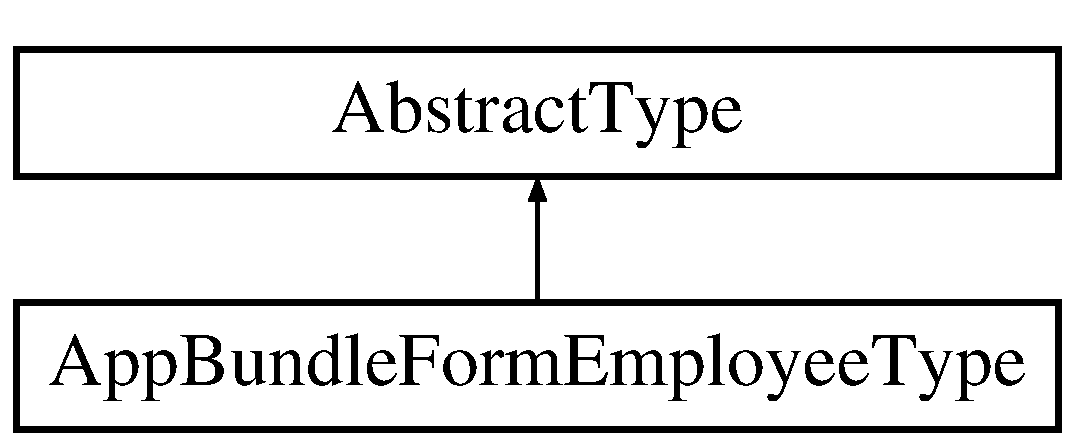
\includegraphics[height=2.000000cm]{class_app_bundle_1_1_form_1_1_employee_type}
\end{center}
\end{figure}
\subsection*{Public Member Functions}
\begin{DoxyCompactItemize}
\item 
\mbox{\hyperlink{class_app_bundle_1_1_form_1_1_employee_type_a040f771cf8a566d92f192a256fa2abe5}{build\+Form}} (Form\+Builder\+Interface \$builder, array \$options)
\item 
\mbox{\hyperlink{class_app_bundle_1_1_form_1_1_employee_type_a09552cba014fd6ff78910a1797099522}{configure\+Options}} (Options\+Resolver \$resolver)
\item 
\mbox{\hyperlink{class_app_bundle_1_1_form_1_1_employee_type_a4ebe090c2e4427b91372e9cdc6b935f0}{get\+Block\+Prefix}} ()
\end{DoxyCompactItemize}


\subsection{Member Function Documentation}
\mbox{\Hypertarget{class_app_bundle_1_1_form_1_1_employee_type_a040f771cf8a566d92f192a256fa2abe5}\label{class_app_bundle_1_1_form_1_1_employee_type_a040f771cf8a566d92f192a256fa2abe5}} 
\index{App\+Bundle\+::\+Form\+::\+Employee\+Type@{App\+Bundle\+::\+Form\+::\+Employee\+Type}!build\+Form@{build\+Form}}
\index{build\+Form@{build\+Form}!App\+Bundle\+::\+Form\+::\+Employee\+Type@{App\+Bundle\+::\+Form\+::\+Employee\+Type}}
\subsubsection{\texorpdfstring{build\+Form()}{buildForm()}}
{\footnotesize\ttfamily App\+Bundle\textbackslash{}\+Form\textbackslash{}\+Employee\+Type\+::build\+Form (\begin{DoxyParamCaption}\item[{Form\+Builder\+Interface}]{\$builder,  }\item[{array}]{\$options }\end{DoxyParamCaption})}

\{\} \mbox{\Hypertarget{class_app_bundle_1_1_form_1_1_employee_type_a09552cba014fd6ff78910a1797099522}\label{class_app_bundle_1_1_form_1_1_employee_type_a09552cba014fd6ff78910a1797099522}} 
\index{App\+Bundle\+::\+Form\+::\+Employee\+Type@{App\+Bundle\+::\+Form\+::\+Employee\+Type}!configure\+Options@{configure\+Options}}
\index{configure\+Options@{configure\+Options}!App\+Bundle\+::\+Form\+::\+Employee\+Type@{App\+Bundle\+::\+Form\+::\+Employee\+Type}}
\subsubsection{\texorpdfstring{configure\+Options()}{configureOptions()}}
{\footnotesize\ttfamily App\+Bundle\textbackslash{}\+Form\textbackslash{}\+Employee\+Type\+::configure\+Options (\begin{DoxyParamCaption}\item[{Options\+Resolver}]{\$resolver }\end{DoxyParamCaption})}

\{\} \mbox{\Hypertarget{class_app_bundle_1_1_form_1_1_employee_type_a4ebe090c2e4427b91372e9cdc6b935f0}\label{class_app_bundle_1_1_form_1_1_employee_type_a4ebe090c2e4427b91372e9cdc6b935f0}} 
\index{App\+Bundle\+::\+Form\+::\+Employee\+Type@{App\+Bundle\+::\+Form\+::\+Employee\+Type}!get\+Block\+Prefix@{get\+Block\+Prefix}}
\index{get\+Block\+Prefix@{get\+Block\+Prefix}!App\+Bundle\+::\+Form\+::\+Employee\+Type@{App\+Bundle\+::\+Form\+::\+Employee\+Type}}
\subsubsection{\texorpdfstring{get\+Block\+Prefix()}{getBlockPrefix()}}
{\footnotesize\ttfamily App\+Bundle\textbackslash{}\+Form\textbackslash{}\+Employee\+Type\+::get\+Block\+Prefix (\begin{DoxyParamCaption}{ }\end{DoxyParamCaption})}

\{\} 

The documentation for this class was generated from the following file\+:\begin{DoxyCompactItemize}
\item 
src/\+App\+Bundle/\+Form/Employee\+Type.\+php\end{DoxyCompactItemize}

\hypertarget{class_app_bundle_1_1_entity_1_1_environment}{}\section{App\+Bundle\textbackslash{}Entity\textbackslash{}Environment Class Reference}
\label{class_app_bundle_1_1_entity_1_1_environment}\index{App\+Bundle\textbackslash{}\+Entity\textbackslash{}\+Environment@{App\+Bundle\textbackslash{}\+Entity\textbackslash{}\+Environment}}
\subsection*{Public Member Functions}
\begin{DoxyCompactItemize}
\item 
\mbox{\hyperlink{class_app_bundle_1_1_entity_1_1_environment_a64c10b203ad4c23205d9f53ec7f66e63}{get\+Id}} ()
\item 
\mbox{\hyperlink{class_app_bundle_1_1_entity_1_1_environment_a8b571562ffee574942b807c92e7de3b4}{set\+Building}} (\$building)
\item 
\mbox{\hyperlink{class_app_bundle_1_1_entity_1_1_environment_a86fd85af01868fe93f4d35775c265c5c}{get\+Building}} ()
\item 
\mbox{\hyperlink{class_app_bundle_1_1_entity_1_1_environment_a8993cc1bedd743e58c3eed6b23347fe7}{set\+Postal\+Code}} (\$postal\+Code)
\item 
\mbox{\hyperlink{class_app_bundle_1_1_entity_1_1_environment_aaef0918c6dce686a21e50c5a696afe23}{get\+Postal\+Code}} ()
\item 
\mbox{\hyperlink{class_app_bundle_1_1_entity_1_1_environment_a8851f6a5ef9b643eaa5d97d51399e547}{set\+Deskroom}} (\$deskroom)
\item 
\mbox{\hyperlink{class_app_bundle_1_1_entity_1_1_environment_a788745e2b9c4d44ff9c9cb5503e67a30}{get\+Deskroom}} ()
\end{DoxyCompactItemize}


\subsection{Detailed Description}
\mbox{\hyperlink{class_app_bundle_1_1_entity_1_1_environment}{Environment}}

(name=\char`\"{}environment\char`\"{}) (repository\+Class=\char`\"{}\+App\+Bundle\textbackslash{}\+Repository\textbackslash{}\+Environment\+Repository\char`\"{}) 

\subsection{Member Function Documentation}
\mbox{\Hypertarget{class_app_bundle_1_1_entity_1_1_environment_a86fd85af01868fe93f4d35775c265c5c}\label{class_app_bundle_1_1_entity_1_1_environment_a86fd85af01868fe93f4d35775c265c5c}} 
\index{App\+Bundle\+::\+Entity\+::\+Environment@{App\+Bundle\+::\+Entity\+::\+Environment}!get\+Building@{get\+Building}}
\index{get\+Building@{get\+Building}!App\+Bundle\+::\+Entity\+::\+Environment@{App\+Bundle\+::\+Entity\+::\+Environment}}
\subsubsection{\texorpdfstring{get\+Building()}{getBuilding()}}
{\footnotesize\ttfamily App\+Bundle\textbackslash{}\+Entity\textbackslash{}\+Environment\+::get\+Building (\begin{DoxyParamCaption}{ }\end{DoxyParamCaption})}

Get building

\begin{DoxyReturn}{Returns}
string 
\end{DoxyReturn}
\mbox{\Hypertarget{class_app_bundle_1_1_entity_1_1_environment_a788745e2b9c4d44ff9c9cb5503e67a30}\label{class_app_bundle_1_1_entity_1_1_environment_a788745e2b9c4d44ff9c9cb5503e67a30}} 
\index{App\+Bundle\+::\+Entity\+::\+Environment@{App\+Bundle\+::\+Entity\+::\+Environment}!get\+Deskroom@{get\+Deskroom}}
\index{get\+Deskroom@{get\+Deskroom}!App\+Bundle\+::\+Entity\+::\+Environment@{App\+Bundle\+::\+Entity\+::\+Environment}}
\subsubsection{\texorpdfstring{get\+Deskroom()}{getDeskroom()}}
{\footnotesize\ttfamily App\+Bundle\textbackslash{}\+Entity\textbackslash{}\+Environment\+::get\+Deskroom (\begin{DoxyParamCaption}{ }\end{DoxyParamCaption})}

Get deskroom

\begin{DoxyReturn}{Returns}
string 
\end{DoxyReturn}
\mbox{\Hypertarget{class_app_bundle_1_1_entity_1_1_environment_a64c10b203ad4c23205d9f53ec7f66e63}\label{class_app_bundle_1_1_entity_1_1_environment_a64c10b203ad4c23205d9f53ec7f66e63}} 
\index{App\+Bundle\+::\+Entity\+::\+Environment@{App\+Bundle\+::\+Entity\+::\+Environment}!get\+Id@{get\+Id}}
\index{get\+Id@{get\+Id}!App\+Bundle\+::\+Entity\+::\+Environment@{App\+Bundle\+::\+Entity\+::\+Environment}}
\subsubsection{\texorpdfstring{get\+Id()}{getId()}}
{\footnotesize\ttfamily App\+Bundle\textbackslash{}\+Entity\textbackslash{}\+Environment\+::get\+Id (\begin{DoxyParamCaption}{ }\end{DoxyParamCaption})}

Get id

\begin{DoxyReturn}{Returns}
int 
\end{DoxyReturn}
\mbox{\Hypertarget{class_app_bundle_1_1_entity_1_1_environment_aaef0918c6dce686a21e50c5a696afe23}\label{class_app_bundle_1_1_entity_1_1_environment_aaef0918c6dce686a21e50c5a696afe23}} 
\index{App\+Bundle\+::\+Entity\+::\+Environment@{App\+Bundle\+::\+Entity\+::\+Environment}!get\+Postal\+Code@{get\+Postal\+Code}}
\index{get\+Postal\+Code@{get\+Postal\+Code}!App\+Bundle\+::\+Entity\+::\+Environment@{App\+Bundle\+::\+Entity\+::\+Environment}}
\subsubsection{\texorpdfstring{get\+Postal\+Code()}{getPostalCode()}}
{\footnotesize\ttfamily App\+Bundle\textbackslash{}\+Entity\textbackslash{}\+Environment\+::get\+Postal\+Code (\begin{DoxyParamCaption}{ }\end{DoxyParamCaption})}

Get postal\+Code

\begin{DoxyReturn}{Returns}
int 
\end{DoxyReturn}
\mbox{\Hypertarget{class_app_bundle_1_1_entity_1_1_environment_a8b571562ffee574942b807c92e7de3b4}\label{class_app_bundle_1_1_entity_1_1_environment_a8b571562ffee574942b807c92e7de3b4}} 
\index{App\+Bundle\+::\+Entity\+::\+Environment@{App\+Bundle\+::\+Entity\+::\+Environment}!set\+Building@{set\+Building}}
\index{set\+Building@{set\+Building}!App\+Bundle\+::\+Entity\+::\+Environment@{App\+Bundle\+::\+Entity\+::\+Environment}}
\subsubsection{\texorpdfstring{set\+Building()}{setBuilding()}}
{\footnotesize\ttfamily App\+Bundle\textbackslash{}\+Entity\textbackslash{}\+Environment\+::set\+Building (\begin{DoxyParamCaption}\item[{}]{\$building }\end{DoxyParamCaption})}

Set building


\begin{DoxyParams}[1]{Parameters}
string & {\em \$building} & \\
\hline
\end{DoxyParams}
\begin{DoxyReturn}{Returns}
\mbox{\hyperlink{class_app_bundle_1_1_entity_1_1_environment}{Environment}} 
\end{DoxyReturn}
\mbox{\Hypertarget{class_app_bundle_1_1_entity_1_1_environment_a8851f6a5ef9b643eaa5d97d51399e547}\label{class_app_bundle_1_1_entity_1_1_environment_a8851f6a5ef9b643eaa5d97d51399e547}} 
\index{App\+Bundle\+::\+Entity\+::\+Environment@{App\+Bundle\+::\+Entity\+::\+Environment}!set\+Deskroom@{set\+Deskroom}}
\index{set\+Deskroom@{set\+Deskroom}!App\+Bundle\+::\+Entity\+::\+Environment@{App\+Bundle\+::\+Entity\+::\+Environment}}
\subsubsection{\texorpdfstring{set\+Deskroom()}{setDeskroom()}}
{\footnotesize\ttfamily App\+Bundle\textbackslash{}\+Entity\textbackslash{}\+Environment\+::set\+Deskroom (\begin{DoxyParamCaption}\item[{}]{\$deskroom }\end{DoxyParamCaption})}

Set deskroom


\begin{DoxyParams}[1]{Parameters}
string & {\em \$deskroom} & \\
\hline
\end{DoxyParams}
\begin{DoxyReturn}{Returns}
\mbox{\hyperlink{class_app_bundle_1_1_entity_1_1_environment}{Environment}} 
\end{DoxyReturn}
\mbox{\Hypertarget{class_app_bundle_1_1_entity_1_1_environment_a8993cc1bedd743e58c3eed6b23347fe7}\label{class_app_bundle_1_1_entity_1_1_environment_a8993cc1bedd743e58c3eed6b23347fe7}} 
\index{App\+Bundle\+::\+Entity\+::\+Environment@{App\+Bundle\+::\+Entity\+::\+Environment}!set\+Postal\+Code@{set\+Postal\+Code}}
\index{set\+Postal\+Code@{set\+Postal\+Code}!App\+Bundle\+::\+Entity\+::\+Environment@{App\+Bundle\+::\+Entity\+::\+Environment}}
\subsubsection{\texorpdfstring{set\+Postal\+Code()}{setPostalCode()}}
{\footnotesize\ttfamily App\+Bundle\textbackslash{}\+Entity\textbackslash{}\+Environment\+::set\+Postal\+Code (\begin{DoxyParamCaption}\item[{}]{\$postal\+Code }\end{DoxyParamCaption})}

Set postal\+Code


\begin{DoxyParams}[1]{Parameters}
integer & {\em \$postal\+Code} & \\
\hline
\end{DoxyParams}
\begin{DoxyReturn}{Returns}
\mbox{\hyperlink{class_app_bundle_1_1_entity_1_1_environment}{Environment}} 
\end{DoxyReturn}


The documentation for this class was generated from the following file\+:\begin{DoxyCompactItemize}
\item 
src/\+App\+Bundle/\+Entity/Environment.\+php\end{DoxyCompactItemize}

\hypertarget{class_app_bundle_1_1_repository_1_1_environment_repository}{}\section{App\+Bundle\textbackslash{}Repository\textbackslash{}Environment\+Repository Class Reference}
\label{class_app_bundle_1_1_repository_1_1_environment_repository}\index{App\+Bundle\textbackslash{}\+Repository\textbackslash{}\+Environment\+Repository@{App\+Bundle\textbackslash{}\+Repository\textbackslash{}\+Environment\+Repository}}
Inheritance diagram for App\+Bundle\textbackslash{}Repository\textbackslash{}Environment\+Repository\+:\begin{figure}[H]
\begin{center}
\leavevmode
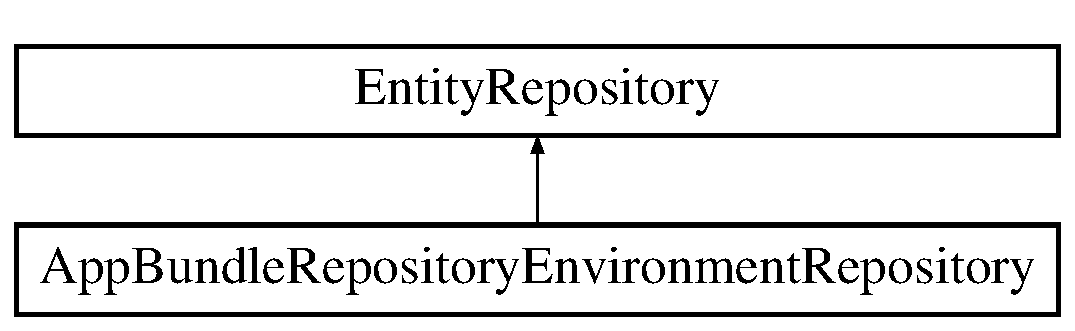
\includegraphics[height=2.000000cm]{class_app_bundle_1_1_repository_1_1_environment_repository}
\end{center}
\end{figure}


\subsection{Detailed Description}
\mbox{\hyperlink{class_app_bundle_1_1_repository_1_1_environment_repository}{Environment\+Repository}}

This class was generated by the Doctrine O\+RM. Add your own custom repository methods below. 

The documentation for this class was generated from the following file\+:\begin{DoxyCompactItemize}
\item 
src/\+App\+Bundle/\+Repository/Environment\+Repository.\+php\end{DoxyCompactItemize}

\hypertarget{class_app_bundle_1_1_form_1_1_environment_type}{}\section{App\+Bundle\textbackslash{}Form\textbackslash{}Environment\+Type Class Reference}
\label{class_app_bundle_1_1_form_1_1_environment_type}\index{App\+Bundle\textbackslash{}\+Form\textbackslash{}\+Environment\+Type@{App\+Bundle\textbackslash{}\+Form\textbackslash{}\+Environment\+Type}}
Inheritance diagram for App\+Bundle\textbackslash{}Form\textbackslash{}Environment\+Type\+:\begin{figure}[H]
\begin{center}
\leavevmode
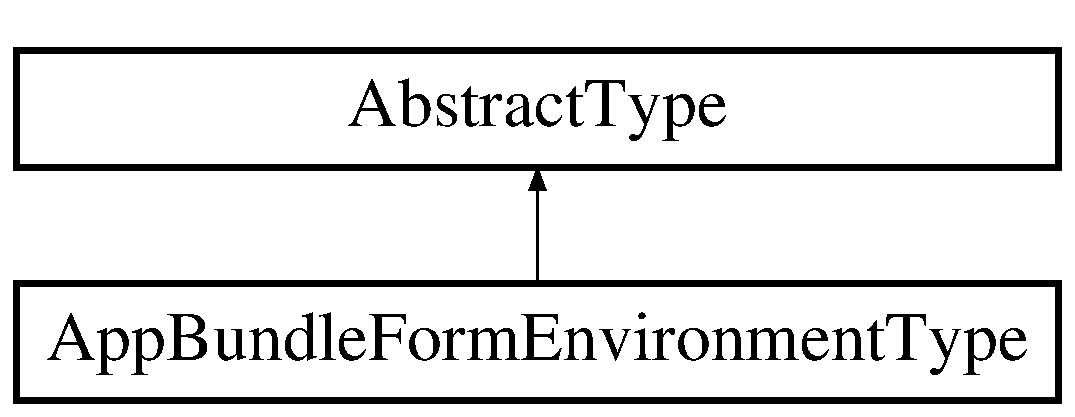
\includegraphics[height=2.000000cm]{class_app_bundle_1_1_form_1_1_environment_type}
\end{center}
\end{figure}
\subsection*{Public Member Functions}
\begin{DoxyCompactItemize}
\item 
\mbox{\hyperlink{class_app_bundle_1_1_form_1_1_environment_type_a49d73fc4e3bf25cf670324750c957c7a}{build\+Form}} (Form\+Builder\+Interface \$builder, array \$options)
\item 
\mbox{\hyperlink{class_app_bundle_1_1_form_1_1_environment_type_a2c5f467c89b99ebdec89fef68deb0838}{configure\+Options}} (Options\+Resolver \$resolver)
\item 
\mbox{\hyperlink{class_app_bundle_1_1_form_1_1_environment_type_a3b35f48ddd80f83d78a2f0cc5814d5fb}{get\+Block\+Prefix}} ()
\end{DoxyCompactItemize}


\subsection{Member Function Documentation}
\mbox{\Hypertarget{class_app_bundle_1_1_form_1_1_environment_type_a49d73fc4e3bf25cf670324750c957c7a}\label{class_app_bundle_1_1_form_1_1_environment_type_a49d73fc4e3bf25cf670324750c957c7a}} 
\index{App\+Bundle\+::\+Form\+::\+Environment\+Type@{App\+Bundle\+::\+Form\+::\+Environment\+Type}!build\+Form@{build\+Form}}
\index{build\+Form@{build\+Form}!App\+Bundle\+::\+Form\+::\+Environment\+Type@{App\+Bundle\+::\+Form\+::\+Environment\+Type}}
\subsubsection{\texorpdfstring{build\+Form()}{buildForm()}}
{\footnotesize\ttfamily App\+Bundle\textbackslash{}\+Form\textbackslash{}\+Environment\+Type\+::build\+Form (\begin{DoxyParamCaption}\item[{Form\+Builder\+Interface}]{\$builder,  }\item[{array}]{\$options }\end{DoxyParamCaption})}

\{\} \mbox{\Hypertarget{class_app_bundle_1_1_form_1_1_environment_type_a2c5f467c89b99ebdec89fef68deb0838}\label{class_app_bundle_1_1_form_1_1_environment_type_a2c5f467c89b99ebdec89fef68deb0838}} 
\index{App\+Bundle\+::\+Form\+::\+Environment\+Type@{App\+Bundle\+::\+Form\+::\+Environment\+Type}!configure\+Options@{configure\+Options}}
\index{configure\+Options@{configure\+Options}!App\+Bundle\+::\+Form\+::\+Environment\+Type@{App\+Bundle\+::\+Form\+::\+Environment\+Type}}
\subsubsection{\texorpdfstring{configure\+Options()}{configureOptions()}}
{\footnotesize\ttfamily App\+Bundle\textbackslash{}\+Form\textbackslash{}\+Environment\+Type\+::configure\+Options (\begin{DoxyParamCaption}\item[{Options\+Resolver}]{\$resolver }\end{DoxyParamCaption})}

\{\} \mbox{\Hypertarget{class_app_bundle_1_1_form_1_1_environment_type_a3b35f48ddd80f83d78a2f0cc5814d5fb}\label{class_app_bundle_1_1_form_1_1_environment_type_a3b35f48ddd80f83d78a2f0cc5814d5fb}} 
\index{App\+Bundle\+::\+Form\+::\+Environment\+Type@{App\+Bundle\+::\+Form\+::\+Environment\+Type}!get\+Block\+Prefix@{get\+Block\+Prefix}}
\index{get\+Block\+Prefix@{get\+Block\+Prefix}!App\+Bundle\+::\+Form\+::\+Environment\+Type@{App\+Bundle\+::\+Form\+::\+Environment\+Type}}
\subsubsection{\texorpdfstring{get\+Block\+Prefix()}{getBlockPrefix()}}
{\footnotesize\ttfamily App\+Bundle\textbackslash{}\+Form\textbackslash{}\+Environment\+Type\+::get\+Block\+Prefix (\begin{DoxyParamCaption}{ }\end{DoxyParamCaption})}

\{\} 

The documentation for this class was generated from the following file\+:\begin{DoxyCompactItemize}
\item 
src/\+App\+Bundle/\+Form/Environment\+Type.\+php\end{DoxyCompactItemize}

\hypertarget{class_app_bundle_1_1_controller_1_1_list_controller}{}\section{App\+Bundle\textbackslash{}Controller\textbackslash{}List\+Controller Class Reference}
\label{class_app_bundle_1_1_controller_1_1_list_controller}\index{App\+Bundle\textbackslash{}\+Controller\textbackslash{}\+List\+Controller@{App\+Bundle\textbackslash{}\+Controller\textbackslash{}\+List\+Controller}}
Inheritance diagram for App\+Bundle\textbackslash{}Controller\textbackslash{}List\+Controller\+:\begin{figure}[H]
\begin{center}
\leavevmode
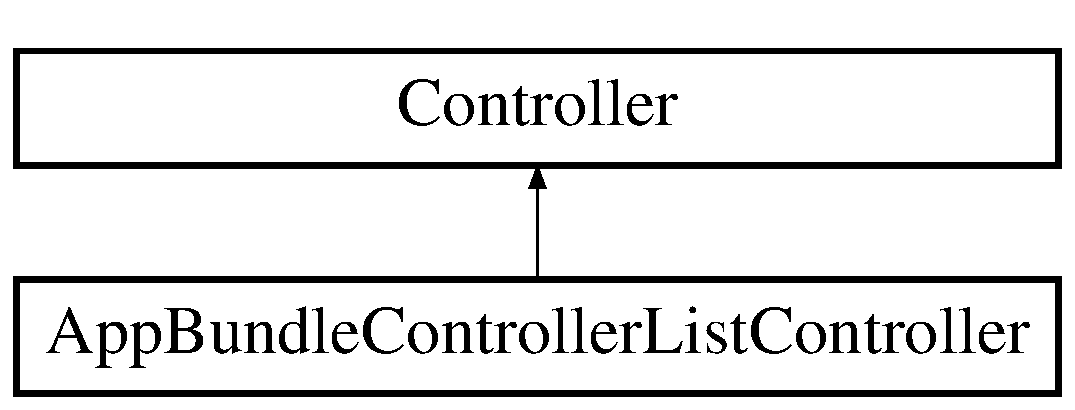
\includegraphics[height=2.000000cm]{class_app_bundle_1_1_controller_1_1_list_controller}
\end{center}
\end{figure}
\subsection*{Public Member Functions}
\begin{DoxyCompactItemize}
\item 
\mbox{\hyperlink{class_app_bundle_1_1_controller_1_1_list_controller_a6df066ca96b72968bf40cfed9d58a010}{list\+Employees\+Action}} (Request \$request)
\end{DoxyCompactItemize}


\subsection{Member Function Documentation}
\mbox{\Hypertarget{class_app_bundle_1_1_controller_1_1_list_controller_a6df066ca96b72968bf40cfed9d58a010}\label{class_app_bundle_1_1_controller_1_1_list_controller_a6df066ca96b72968bf40cfed9d58a010}} 
\index{App\+Bundle\+::\+Controller\+::\+List\+Controller@{App\+Bundle\+::\+Controller\+::\+List\+Controller}!list\+Employees\+Action@{list\+Employees\+Action}}
\index{list\+Employees\+Action@{list\+Employees\+Action}!App\+Bundle\+::\+Controller\+::\+List\+Controller@{App\+Bundle\+::\+Controller\+::\+List\+Controller}}
\subsubsection{\texorpdfstring{list\+Employees\+Action()}{listEmployeesAction()}}
{\footnotesize\ttfamily App\+Bundle\textbackslash{}\+Controller\textbackslash{}\+List\+Controller\+::list\+Employees\+Action (\begin{DoxyParamCaption}\item[{Request}]{\$request }\end{DoxyParamCaption})}

(\char`\"{}/list\char`\"{}, name=\char`\"{}list\char`\"{}) (\char`\"{}has\+\_\+role(\textquotesingle{}\+R\+O\+L\+E\+\_\+\+U\+S\+E\+R\textquotesingle{}) or has\+\_\+role(\textquotesingle{}\+R\+O\+L\+E\+\_\+\+A\+D\+M\+I\+N\textquotesingle{})\char`\"{}) 

The documentation for this class was generated from the following file\+:\begin{DoxyCompactItemize}
\item 
src/\+App\+Bundle/\+Controller/List\+Controller.\+php\end{DoxyCompactItemize}

\hypertarget{class_app_bundle_1_1_controller_1_1_login_controller}{}\section{App\+Bundle\textbackslash{}Controller\textbackslash{}Login\+Controller Class Reference}
\label{class_app_bundle_1_1_controller_1_1_login_controller}\index{App\+Bundle\textbackslash{}\+Controller\textbackslash{}\+Login\+Controller@{App\+Bundle\textbackslash{}\+Controller\textbackslash{}\+Login\+Controller}}
Inheritance diagram for App\+Bundle\textbackslash{}Controller\textbackslash{}Login\+Controller\+:\begin{figure}[H]
\begin{center}
\leavevmode
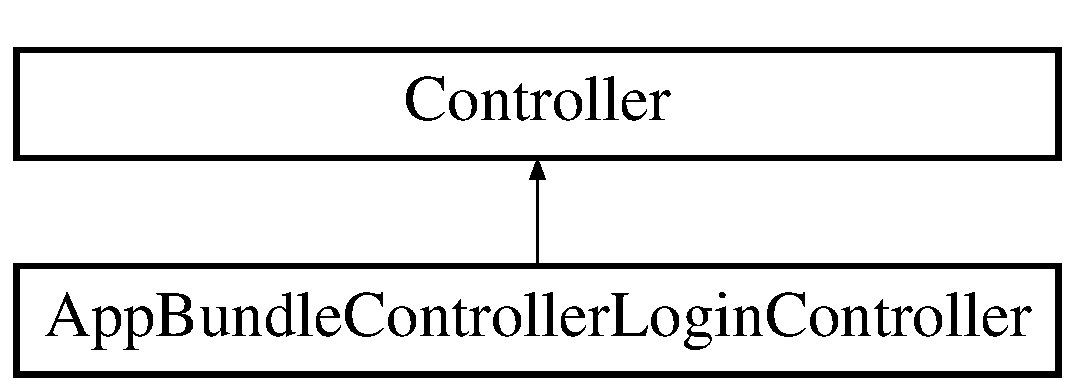
\includegraphics[height=2.000000cm]{class_app_bundle_1_1_controller_1_1_login_controller}
\end{center}
\end{figure}
\subsection*{Public Member Functions}
\begin{DoxyCompactItemize}
\item 
\mbox{\hyperlink{class_app_bundle_1_1_controller_1_1_login_controller_a263f12317c12ef52590611074ddae532}{index\+Action}} ()
\end{DoxyCompactItemize}


\subsection{Member Function Documentation}
\mbox{\Hypertarget{class_app_bundle_1_1_controller_1_1_login_controller_a263f12317c12ef52590611074ddae532}\label{class_app_bundle_1_1_controller_1_1_login_controller_a263f12317c12ef52590611074ddae532}} 
\index{App\+Bundle\+::\+Controller\+::\+Login\+Controller@{App\+Bundle\+::\+Controller\+::\+Login\+Controller}!index\+Action@{index\+Action}}
\index{index\+Action@{index\+Action}!App\+Bundle\+::\+Controller\+::\+Login\+Controller@{App\+Bundle\+::\+Controller\+::\+Login\+Controller}}
\subsubsection{\texorpdfstring{index\+Action()}{indexAction()}}
{\footnotesize\ttfamily App\+Bundle\textbackslash{}\+Controller\textbackslash{}\+Login\+Controller\+::index\+Action (\begin{DoxyParamCaption}{ }\end{DoxyParamCaption})}

(\char`\"{}/\char`\"{}, name=\char`\"{}login\char`\"{}) 

The documentation for this class was generated from the following file\+:\begin{DoxyCompactItemize}
\item 
src/\+App\+Bundle/\+Controller/Login\+Controller.\+php\end{DoxyCompactItemize}

\hypertarget{class_app_bundle_1_1_tests_1_1_controller_1_1_login_controller_test}{}\section{App\+Bundle\textbackslash{}Tests\textbackslash{}Controller\textbackslash{}Login\+Controller\+Test Class Reference}
\label{class_app_bundle_1_1_tests_1_1_controller_1_1_login_controller_test}\index{App\+Bundle\textbackslash{}\+Tests\textbackslash{}\+Controller\textbackslash{}\+Login\+Controller\+Test@{App\+Bundle\textbackslash{}\+Tests\textbackslash{}\+Controller\textbackslash{}\+Login\+Controller\+Test}}
Inheritance diagram for App\+Bundle\textbackslash{}Tests\textbackslash{}Controller\textbackslash{}Login\+Controller\+Test\+:\begin{figure}[H]
\begin{center}
\leavevmode
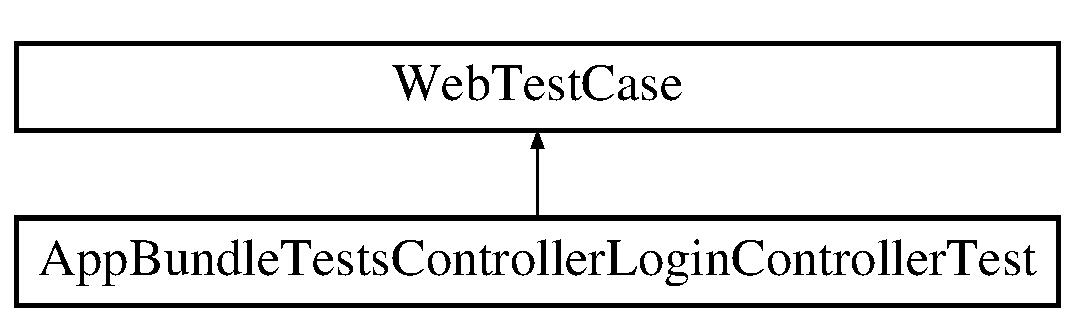
\includegraphics[height=2.000000cm]{class_app_bundle_1_1_tests_1_1_controller_1_1_login_controller_test}
\end{center}
\end{figure}


The documentation for this class was generated from the following file\+:\begin{DoxyCompactItemize}
\item 
src/\+App\+Bundle/\+Tests/\+Controller/Login\+Controller\+Test.\+php\end{DoxyCompactItemize}

\hypertarget{class_app_bundle_1_1_controller_1_1_logout_controller}{}\section{App\+Bundle\textbackslash{}Controller\textbackslash{}Logout\+Controller Class Reference}
\label{class_app_bundle_1_1_controller_1_1_logout_controller}\index{App\+Bundle\textbackslash{}\+Controller\textbackslash{}\+Logout\+Controller@{App\+Bundle\textbackslash{}\+Controller\textbackslash{}\+Logout\+Controller}}
Inheritance diagram for App\+Bundle\textbackslash{}Controller\textbackslash{}Logout\+Controller\+:\begin{figure}[H]
\begin{center}
\leavevmode
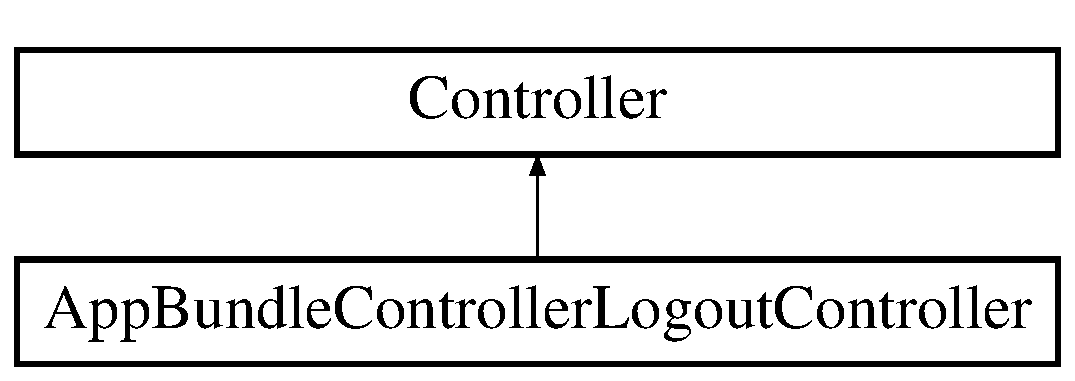
\includegraphics[height=2.000000cm]{class_app_bundle_1_1_controller_1_1_logout_controller}
\end{center}
\end{figure}
\subsection*{Public Member Functions}
\begin{DoxyCompactItemize}
\item 
\mbox{\hyperlink{class_app_bundle_1_1_controller_1_1_logout_controller_ad04fdf5190d7570532321bb806357319}{logout\+Action}} ()
\end{DoxyCompactItemize}


\subsection{Member Function Documentation}
\mbox{\Hypertarget{class_app_bundle_1_1_controller_1_1_logout_controller_ad04fdf5190d7570532321bb806357319}\label{class_app_bundle_1_1_controller_1_1_logout_controller_ad04fdf5190d7570532321bb806357319}} 
\index{App\+Bundle\+::\+Controller\+::\+Logout\+Controller@{App\+Bundle\+::\+Controller\+::\+Logout\+Controller}!logout\+Action@{logout\+Action}}
\index{logout\+Action@{logout\+Action}!App\+Bundle\+::\+Controller\+::\+Logout\+Controller@{App\+Bundle\+::\+Controller\+::\+Logout\+Controller}}
\subsubsection{\texorpdfstring{logout\+Action()}{logoutAction()}}
{\footnotesize\ttfamily App\+Bundle\textbackslash{}\+Controller\textbackslash{}\+Logout\+Controller\+::logout\+Action (\begin{DoxyParamCaption}{ }\end{DoxyParamCaption})}

(\char`\"{}/logout\char`\"{}, name=\char`\"{}logout\char`\"{}) 

The documentation for this class was generated from the following file\+:\begin{DoxyCompactItemize}
\item 
src/\+App\+Bundle/\+Controller/Logout\+Controller.\+php\end{DoxyCompactItemize}

\hypertarget{class_app_bundle_1_1_tests_1_1_controller_1_1_logout_controller_test}{}\section{App\+Bundle\textbackslash{}Tests\textbackslash{}Controller\textbackslash{}Logout\+Controller\+Test Class Reference}
\label{class_app_bundle_1_1_tests_1_1_controller_1_1_logout_controller_test}\index{App\+Bundle\textbackslash{}\+Tests\textbackslash{}\+Controller\textbackslash{}\+Logout\+Controller\+Test@{App\+Bundle\textbackslash{}\+Tests\textbackslash{}\+Controller\textbackslash{}\+Logout\+Controller\+Test}}
Inheritance diagram for App\+Bundle\textbackslash{}Tests\textbackslash{}Controller\textbackslash{}Logout\+Controller\+Test\+:\begin{figure}[H]
\begin{center}
\leavevmode
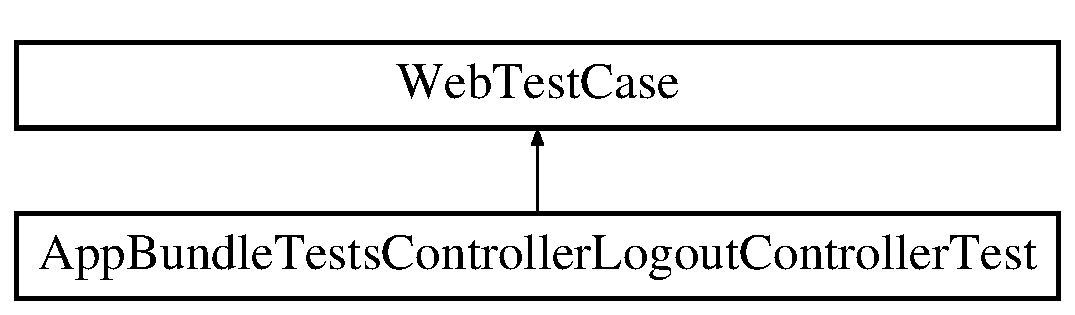
\includegraphics[height=2.000000cm]{class_app_bundle_1_1_tests_1_1_controller_1_1_logout_controller_test}
\end{center}
\end{figure}


The documentation for this class was generated from the following file\+:\begin{DoxyCompactItemize}
\item 
src/\+App\+Bundle/\+Tests/\+Controller/Logout\+Controller\+Test.\+php\end{DoxyCompactItemize}

\hypertarget{class_app_bundle_1_1_entity_1_1_skill}{}\section{App\+Bundle\textbackslash{}Entity\textbackslash{}Skill Class Reference}
\label{class_app_bundle_1_1_entity_1_1_skill}\index{App\+Bundle\textbackslash{}\+Entity\textbackslash{}\+Skill@{App\+Bundle\textbackslash{}\+Entity\textbackslash{}\+Skill}}
\subsection*{Public Member Functions}
\begin{DoxyCompactItemize}
\item 
\mbox{\hyperlink{class_app_bundle_1_1_entity_1_1_skill_a46db4431c15f4d2a9a7e2a8055cfbd15}{get\+Id}} ()
\item 
\mbox{\hyperlink{class_app_bundle_1_1_entity_1_1_skill_ac6d7d4286476c5d583d190533e9425a6}{set\+Denomination}} (\$denomination)
\item 
\mbox{\hyperlink{class_app_bundle_1_1_entity_1_1_skill_a32de8d5ba9615669a191a77cec3bbf48}{get\+Denomination}} ()
\item 
\mbox{\hyperlink{class_app_bundle_1_1_entity_1_1_skill_a8c92b9e81fa71efafd400645b4adb1b8}{set\+Employee}} (\textbackslash{}\mbox{\hyperlink{class_app_bundle_1_1_entity_1_1_employee}{App\+Bundle\textbackslash{}\+Entity\textbackslash{}\+Employee}} \$employee=null)
\item 
\mbox{\hyperlink{class_app_bundle_1_1_entity_1_1_skill_a51b3c9c44296f130bd2a988e1f399fc2}{get\+Employee}} ()
\end{DoxyCompactItemize}


\subsection{Detailed Description}
Skills

(name=\char`\"{}skills\char`\"{}) (repository\+Class=\char`\"{}\+App\+Bundle\textbackslash{}\+Repository\textbackslash{}\+Skills\+Repository\char`\"{}) 

\subsection{Member Function Documentation}
\mbox{\Hypertarget{class_app_bundle_1_1_entity_1_1_skill_a32de8d5ba9615669a191a77cec3bbf48}\label{class_app_bundle_1_1_entity_1_1_skill_a32de8d5ba9615669a191a77cec3bbf48}} 
\index{App\+Bundle\+::\+Entity\+::\+Skill@{App\+Bundle\+::\+Entity\+::\+Skill}!get\+Denomination@{get\+Denomination}}
\index{get\+Denomination@{get\+Denomination}!App\+Bundle\+::\+Entity\+::\+Skill@{App\+Bundle\+::\+Entity\+::\+Skill}}
\subsubsection{\texorpdfstring{get\+Denomination()}{getDenomination()}}
{\footnotesize\ttfamily App\+Bundle\textbackslash{}\+Entity\textbackslash{}\+Skill\+::get\+Denomination (\begin{DoxyParamCaption}{ }\end{DoxyParamCaption})}

Get denomination

\begin{DoxyReturn}{Returns}
string 
\end{DoxyReturn}
\mbox{\Hypertarget{class_app_bundle_1_1_entity_1_1_skill_a51b3c9c44296f130bd2a988e1f399fc2}\label{class_app_bundle_1_1_entity_1_1_skill_a51b3c9c44296f130bd2a988e1f399fc2}} 
\index{App\+Bundle\+::\+Entity\+::\+Skill@{App\+Bundle\+::\+Entity\+::\+Skill}!get\+Employee@{get\+Employee}}
\index{get\+Employee@{get\+Employee}!App\+Bundle\+::\+Entity\+::\+Skill@{App\+Bundle\+::\+Entity\+::\+Skill}}
\subsubsection{\texorpdfstring{get\+Employee()}{getEmployee()}}
{\footnotesize\ttfamily App\+Bundle\textbackslash{}\+Entity\textbackslash{}\+Skill\+::get\+Employee (\begin{DoxyParamCaption}{ }\end{DoxyParamCaption})}

Get employee

\begin{DoxyReturn}{Returns}

\end{DoxyReturn}
\mbox{\Hypertarget{class_app_bundle_1_1_entity_1_1_skill_a46db4431c15f4d2a9a7e2a8055cfbd15}\label{class_app_bundle_1_1_entity_1_1_skill_a46db4431c15f4d2a9a7e2a8055cfbd15}} 
\index{App\+Bundle\+::\+Entity\+::\+Skill@{App\+Bundle\+::\+Entity\+::\+Skill}!get\+Id@{get\+Id}}
\index{get\+Id@{get\+Id}!App\+Bundle\+::\+Entity\+::\+Skill@{App\+Bundle\+::\+Entity\+::\+Skill}}
\subsubsection{\texorpdfstring{get\+Id()}{getId()}}
{\footnotesize\ttfamily App\+Bundle\textbackslash{}\+Entity\textbackslash{}\+Skill\+::get\+Id (\begin{DoxyParamCaption}{ }\end{DoxyParamCaption})}

Get id

\begin{DoxyReturn}{Returns}
int 
\end{DoxyReturn}
\mbox{\Hypertarget{class_app_bundle_1_1_entity_1_1_skill_ac6d7d4286476c5d583d190533e9425a6}\label{class_app_bundle_1_1_entity_1_1_skill_ac6d7d4286476c5d583d190533e9425a6}} 
\index{App\+Bundle\+::\+Entity\+::\+Skill@{App\+Bundle\+::\+Entity\+::\+Skill}!set\+Denomination@{set\+Denomination}}
\index{set\+Denomination@{set\+Denomination}!App\+Bundle\+::\+Entity\+::\+Skill@{App\+Bundle\+::\+Entity\+::\+Skill}}
\subsubsection{\texorpdfstring{set\+Denomination()}{setDenomination()}}
{\footnotesize\ttfamily App\+Bundle\textbackslash{}\+Entity\textbackslash{}\+Skill\+::set\+Denomination (\begin{DoxyParamCaption}\item[{}]{\$denomination }\end{DoxyParamCaption})}

Set denomination


\begin{DoxyParams}[1]{Parameters}
string & {\em \$denomination} & \\
\hline
\end{DoxyParams}
\begin{DoxyReturn}{Returns}
\mbox{\hyperlink{class_app_bundle_1_1_entity_1_1_skill}{Skill}} 
\end{DoxyReturn}
\mbox{\Hypertarget{class_app_bundle_1_1_entity_1_1_skill_a8c92b9e81fa71efafd400645b4adb1b8}\label{class_app_bundle_1_1_entity_1_1_skill_a8c92b9e81fa71efafd400645b4adb1b8}} 
\index{App\+Bundle\+::\+Entity\+::\+Skill@{App\+Bundle\+::\+Entity\+::\+Skill}!set\+Employee@{set\+Employee}}
\index{set\+Employee@{set\+Employee}!App\+Bundle\+::\+Entity\+::\+Skill@{App\+Bundle\+::\+Entity\+::\+Skill}}
\subsubsection{\texorpdfstring{set\+Employee()}{setEmployee()}}
{\footnotesize\ttfamily App\+Bundle\textbackslash{}\+Entity\textbackslash{}\+Skill\+::set\+Employee (\begin{DoxyParamCaption}\item[{\textbackslash{}\mbox{\hyperlink{class_app_bundle_1_1_entity_1_1_employee}{App\+Bundle\textbackslash{}\+Entity\textbackslash{}\+Employee}}}]{\$employee = {\ttfamily null} }\end{DoxyParamCaption})}

Set employee


\begin{DoxyParams}[1]{Parameters}
\textbackslash{}\+App\+Bundle\textbackslash{}\+Entity\textbackslash{}\+Employee & {\em \$employee} & \\
\hline
\end{DoxyParams}
\begin{DoxyReturn}{Returns}
\mbox{\hyperlink{class_app_bundle_1_1_entity_1_1_skill}{Skill}} 
\end{DoxyReturn}


The documentation for this class was generated from the following file\+:\begin{DoxyCompactItemize}
\item 
src/\+App\+Bundle/\+Entity/Skill.\+php\end{DoxyCompactItemize}

\hypertarget{class_app_bundle_1_1_repository_1_1_skills_repository}{}\section{App\+Bundle\textbackslash{}Repository\textbackslash{}Skills\+Repository Class Reference}
\label{class_app_bundle_1_1_repository_1_1_skills_repository}\index{App\+Bundle\textbackslash{}\+Repository\textbackslash{}\+Skills\+Repository@{App\+Bundle\textbackslash{}\+Repository\textbackslash{}\+Skills\+Repository}}
Inheritance diagram for App\+Bundle\textbackslash{}Repository\textbackslash{}Skills\+Repository\+:\begin{figure}[H]
\begin{center}
\leavevmode
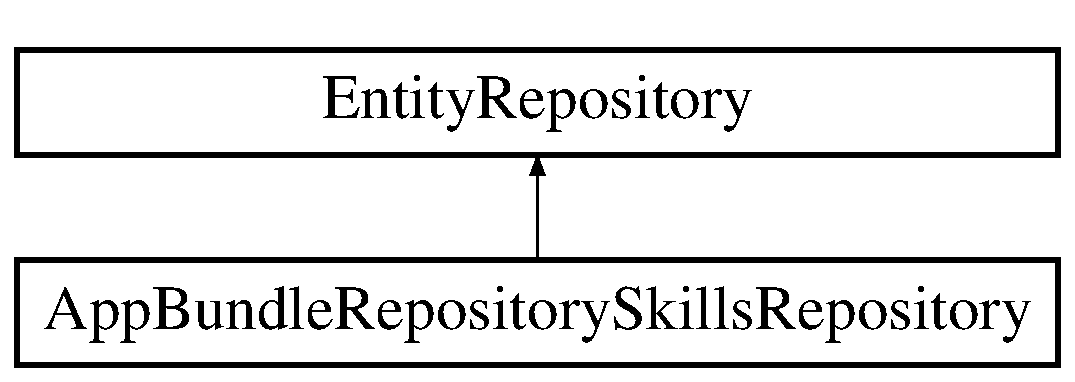
\includegraphics[height=2.000000cm]{class_app_bundle_1_1_repository_1_1_skills_repository}
\end{center}
\end{figure}


\subsection{Detailed Description}
\mbox{\hyperlink{class_app_bundle_1_1_repository_1_1_skills_repository}{Skills\+Repository}}

This class was generated by the Doctrine O\+RM. Add your own custom repository methods below. 

The documentation for this class was generated from the following file\+:\begin{DoxyCompactItemize}
\item 
src/\+App\+Bundle/\+Repository/Skills\+Repository.\+php\end{DoxyCompactItemize}

\hypertarget{class_app_bundle_1_1_form_1_1_skill_type}{}\section{App\+Bundle\textbackslash{}Form\textbackslash{}Skill\+Type Class Reference}
\label{class_app_bundle_1_1_form_1_1_skill_type}\index{App\+Bundle\textbackslash{}\+Form\textbackslash{}\+Skill\+Type@{App\+Bundle\textbackslash{}\+Form\textbackslash{}\+Skill\+Type}}
Inheritance diagram for App\+Bundle\textbackslash{}Form\textbackslash{}Skill\+Type\+:\begin{figure}[H]
\begin{center}
\leavevmode
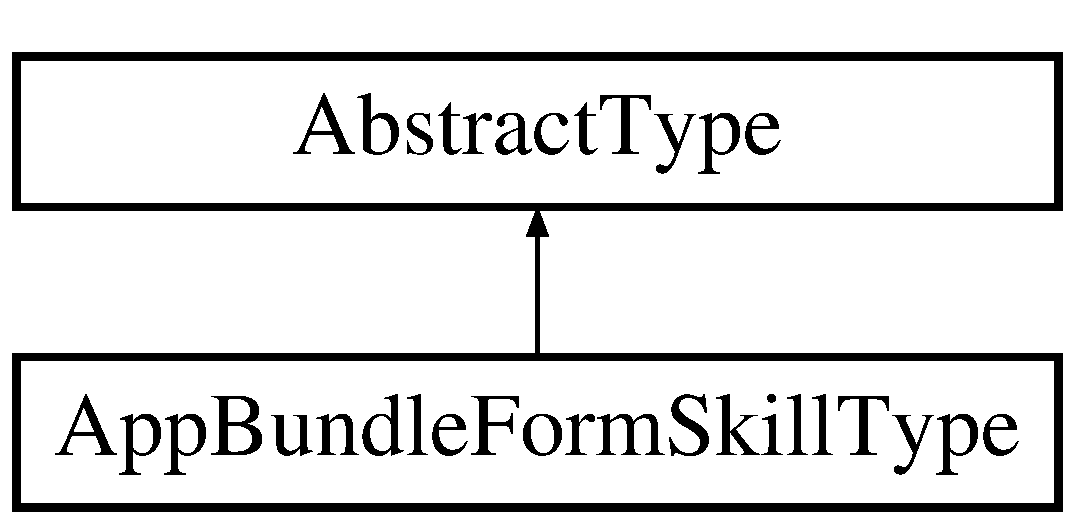
\includegraphics[height=2.000000cm]{class_app_bundle_1_1_form_1_1_skill_type}
\end{center}
\end{figure}
\subsection*{Public Member Functions}
\begin{DoxyCompactItemize}
\item 
\mbox{\hyperlink{class_app_bundle_1_1_form_1_1_skill_type_a849b17cb441eee94c23e849ad54acf7a}{build\+Form}} (Form\+Builder\+Interface \$builder, array \$options)
\item 
\mbox{\hyperlink{class_app_bundle_1_1_form_1_1_skill_type_aaebaf3b685fa968a94a4cd89fca72a9f}{configure\+Options}} (Options\+Resolver \$resolver)
\item 
\mbox{\hyperlink{class_app_bundle_1_1_form_1_1_skill_type_a40d9ea856188ed3c84fb1453d9b521f3}{get\+Block\+Prefix}} ()
\end{DoxyCompactItemize}


\subsection{Member Function Documentation}
\mbox{\Hypertarget{class_app_bundle_1_1_form_1_1_skill_type_a849b17cb441eee94c23e849ad54acf7a}\label{class_app_bundle_1_1_form_1_1_skill_type_a849b17cb441eee94c23e849ad54acf7a}} 
\index{App\+Bundle\+::\+Form\+::\+Skill\+Type@{App\+Bundle\+::\+Form\+::\+Skill\+Type}!build\+Form@{build\+Form}}
\index{build\+Form@{build\+Form}!App\+Bundle\+::\+Form\+::\+Skill\+Type@{App\+Bundle\+::\+Form\+::\+Skill\+Type}}
\subsubsection{\texorpdfstring{build\+Form()}{buildForm()}}
{\footnotesize\ttfamily App\+Bundle\textbackslash{}\+Form\textbackslash{}\+Skill\+Type\+::build\+Form (\begin{DoxyParamCaption}\item[{Form\+Builder\+Interface}]{\$builder,  }\item[{array}]{\$options }\end{DoxyParamCaption})}

\{\} \mbox{\Hypertarget{class_app_bundle_1_1_form_1_1_skill_type_aaebaf3b685fa968a94a4cd89fca72a9f}\label{class_app_bundle_1_1_form_1_1_skill_type_aaebaf3b685fa968a94a4cd89fca72a9f}} 
\index{App\+Bundle\+::\+Form\+::\+Skill\+Type@{App\+Bundle\+::\+Form\+::\+Skill\+Type}!configure\+Options@{configure\+Options}}
\index{configure\+Options@{configure\+Options}!App\+Bundle\+::\+Form\+::\+Skill\+Type@{App\+Bundle\+::\+Form\+::\+Skill\+Type}}
\subsubsection{\texorpdfstring{configure\+Options()}{configureOptions()}}
{\footnotesize\ttfamily App\+Bundle\textbackslash{}\+Form\textbackslash{}\+Skill\+Type\+::configure\+Options (\begin{DoxyParamCaption}\item[{Options\+Resolver}]{\$resolver }\end{DoxyParamCaption})}

\{\} \mbox{\Hypertarget{class_app_bundle_1_1_form_1_1_skill_type_a40d9ea856188ed3c84fb1453d9b521f3}\label{class_app_bundle_1_1_form_1_1_skill_type_a40d9ea856188ed3c84fb1453d9b521f3}} 
\index{App\+Bundle\+::\+Form\+::\+Skill\+Type@{App\+Bundle\+::\+Form\+::\+Skill\+Type}!get\+Block\+Prefix@{get\+Block\+Prefix}}
\index{get\+Block\+Prefix@{get\+Block\+Prefix}!App\+Bundle\+::\+Form\+::\+Skill\+Type@{App\+Bundle\+::\+Form\+::\+Skill\+Type}}
\subsubsection{\texorpdfstring{get\+Block\+Prefix()}{getBlockPrefix()}}
{\footnotesize\ttfamily App\+Bundle\textbackslash{}\+Form\textbackslash{}\+Skill\+Type\+::get\+Block\+Prefix (\begin{DoxyParamCaption}{ }\end{DoxyParamCaption})}

\{\} 

The documentation for this class was generated from the following file\+:\begin{DoxyCompactItemize}
\item 
src/\+App\+Bundle/\+Form/Skill\+Type.\+php\end{DoxyCompactItemize}

\hypertarget{class_app_bundle_1_1_entity_1_1_user}{}\section{App\+Bundle\textbackslash{}Entity\textbackslash{}User Class Reference}
\label{class_app_bundle_1_1_entity_1_1_user}\index{App\+Bundle\textbackslash{}\+Entity\textbackslash{}\+User@{App\+Bundle\textbackslash{}\+Entity\textbackslash{}\+User}}
Inheritance diagram for App\+Bundle\textbackslash{}Entity\textbackslash{}User\+:\begin{figure}[H]
\begin{center}
\leavevmode
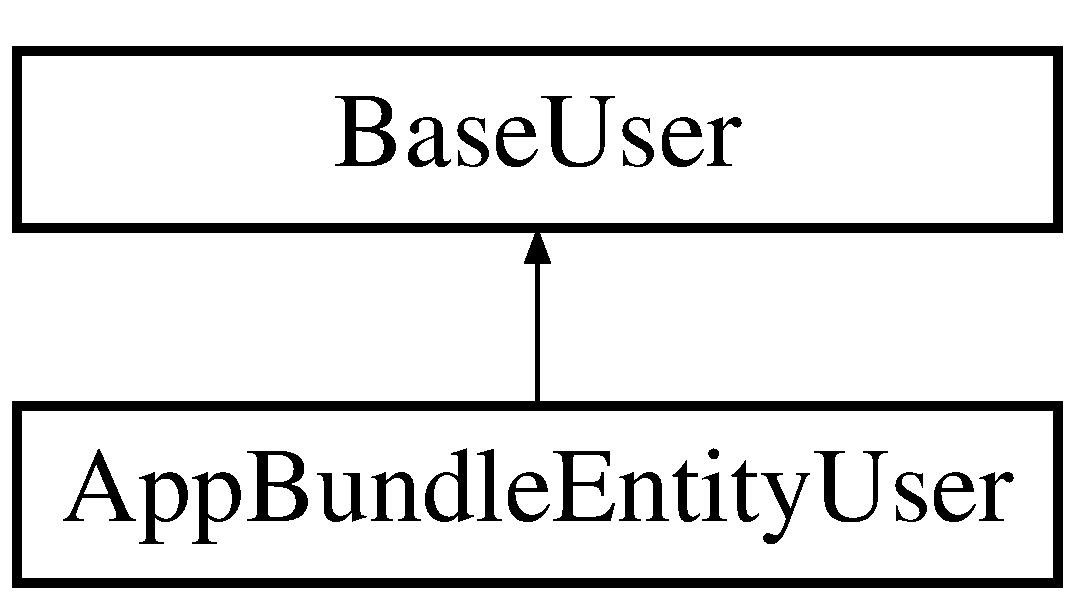
\includegraphics[height=2.000000cm]{class_app_bundle_1_1_entity_1_1_user}
\end{center}
\end{figure}
\subsection*{Protected Attributes}
\begin{DoxyCompactItemize}
\item 
\mbox{\hyperlink{class_app_bundle_1_1_entity_1_1_user_ae12a261b5ca7565baa6c166854cc9860}{\$id}}
\end{DoxyCompactItemize}


\subsection{Detailed Description}
(name=\char`\"{}fos\+\_\+user\char`\"{}) 

\subsection{Member Data Documentation}
\mbox{\Hypertarget{class_app_bundle_1_1_entity_1_1_user_ae12a261b5ca7565baa6c166854cc9860}\label{class_app_bundle_1_1_entity_1_1_user_ae12a261b5ca7565baa6c166854cc9860}} 
\index{App\+Bundle\+::\+Entity\+::\+User@{App\+Bundle\+::\+Entity\+::\+User}!\$id@{\$id}}
\index{\$id@{\$id}!App\+Bundle\+::\+Entity\+::\+User@{App\+Bundle\+::\+Entity\+::\+User}}
\subsubsection{\texorpdfstring{\$id}{$id}}
{\footnotesize\ttfamily App\+Bundle\textbackslash{}\+Entity\textbackslash{}\+User\+::\$id\hspace{0.3cm}{\ttfamily [protected]}}

(type=\char`\"{}integer\char`\"{}) (strategy=\char`\"{}\+A\+U\+T\+O\char`\"{}) 

The documentation for this class was generated from the following file\+:\begin{DoxyCompactItemize}
\item 
src/\+App\+Bundle/\+Entity/User.\+php\end{DoxyCompactItemize}

%--- End generated contents ---

% Index
\backmatter
\newpage
\phantomsection
\clearemptydoublepage
\addcontentsline{toc}{chapter}{Index}
\printindex

\end{document}
